
\chapter{Transformaciones Lineales}

En este capítulo nos interesamos por aquellas aplicaciones entre espacios vectoriales que preservan las operaciones de suma y producto por escalares. Son las aplicaciones o transformaciones lineales. Son las funciones con las que se trabaja en Álgebra Lineal y tienen uma amplia variedad de aplicaciones.  Se verá que, en el caso de dimensión finita,  es posible  asociarles una matriz. Se estudian los espacios asociados; el espacio nulo y el espacio que generan las columnas de la matriz. Un resultado útil e importante es que las sumas de las dimensiones de esos subespacios da la dimensión del espacio de partida. Mostramos la interpretación geométrica tanto de las aplicaciones lineales en el plano como en el espacio. Se presentan una gran variedad de ejemplos.\\
Se  estudia, además, el espacio dual de un espacio vectorial. Es el conjunto de todas las transformaciones lineales entre un espacio vectorial y el cuerpo de los escalares, conocidas como funcionales lineales. 
%Las transformaciones (o aplicaciones) lineales son las funciones con las que se trabaja en Algebra Lineal. Son funciones que van de un %espacio vectorial a otro y tienen una gran variedad de aplicaciones.

\section{Definición de transformación lineal. Ejemplos.}

\bigskip

\begin{definition}\label{TL}\index{Transformación lineal}


Sean $V$ y $W$ dos espacios vectoriales, una \textit{transformación lineal} $T$ de $V$ en $W$ es una aplicación $T: V \rightarrow W$ tal que: 


\bigskip

\begin{enumerate}

\item $T(\vec{v}+\vec{w})=T(\vec{v})+T(\vec{w})$ para todo  $\vec{v}$, $\vec{w}$ $\in V$.

\item $T(a ~\vec{v})=a~T(\vec{v})$ para todo $a\in K$ y todo $\vec{v}$ $\in V$.
  

\end{enumerate}

\end{definition}

\bigskip

\bigskip

Entre las transformaciones lineales más utilizadas están las proyecciones. En la Figura \ref{figproyxy} se muestra la proyección ortogonal  de un vector $\vec{v}=(x,y,z)$ sobre el plano $xy$. \index{Proyección ortogonal}

\bigskip

Se tiene $T: \mathbb{R}^3 \rightarrow \mathbb{R}^3$, donde $   T((x,y,z))=(x,y,0)$.
Es una transformación lineal ya que se cumplen para $ \forall ~ \vec{v}=(x,y,z)$, $\vec{w}=(x^{\prime},y^{\prime},z^{\prime})$ y  $ \forall ~a\in K$:



\bigskip

\begin{enumerate}

\item $T(\vec{v}+\vec{w})=T((x+x^{\prime},y+y^{\prime},z+z^{\prime}))= (x+x^{\prime},y+y^{\prime},0) =(x,y,0)+ (x^{\prime},y^{\prime},0)= T(\vec{v})+ T(\vec{w})$.

\bigskip

\item $T(a ~\vec{v})= T( a  (x,y,z)) = T((ax,ay,az)) = (ax,ay,0)=a(x,y,0)=   a~T(\vec{v})$.
  

\end{enumerate}



\bigskip


\begin{figure}[!htbp]
\label{figproyxy}
    \centering
    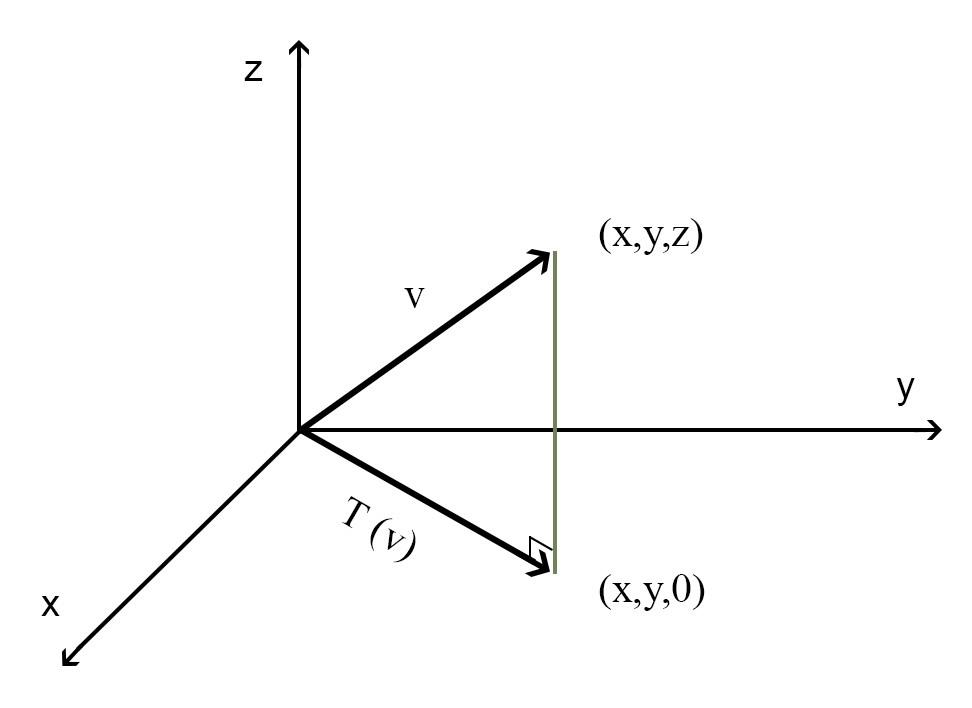
\includegraphics[width=0.60\textwidth]{Pictures/TLfig10.jpg}
    \caption{Proyección ortogonal de un vector $\vec{v}$ sobre el plano $xy$. }
    %\label{TLfig10}
\end{figure}

\begin{remark}
\begin{itemize}
\item En una transformación lineal $V$ y $W$ deben ser espacios vectoriales sobre el mismo cuerpo $K$.

\item Las aplicaciones  $O: V \rightarrow W$, $O(\vec{u})= \vec{0}_W$ para todo $\vec{u} \in V$ y 
$I_d: V \rightarrow V$, $I_d(\vec{u})= \vec{u}$ son  transformaciones lineales.

\item La traza de una matriz, \index{Traza de una matriz}

$Tr: K^{n \times n } \rightarrow K $ dada por $Tr(A)=\sum_{i=1}^n a_{ii}$, es una transformación lineal.



\item $T: \mathbb{R} \rightarrow \mathbb{R}$ dada por $T(x)=x^2$ es un ejemplo de  transformación \textit{no lineal}.
Se tiene que $T(x+y) \neq T(x) + T(y)$, ya que $T(x+y) = (x+y)^2= x^2 + y^2+2xy$,   mientras que $T(x)+T(y) = x^2 + y^2$.
\item
Otro ejemplo de transformación no lineal es el determinante de una matriz, ya que, en general  $Det(A+B) \neq Det(A)+Det(B)$.
\end{itemize}
%\hfill$\blacktriangle$
\end{remark}


\bigskip

\begin{example}
Dado un número real $a$, la aplicación que asocia a cada polinomio $p$ del conjunto  $P_\mathbb{R}\left[t\right]$ su valor en $x=a$, $p(a)$, es una transformación lineal. Está definida mediante las siguientes expresiones: 

$$T: P_\mathbb{R}\left[t\right] \rightarrow \mathbb{R}$$ 

$$T(p(t))=p(a)$$


El hecho que $T$ es una transformación lineal se deduce de las igualdades $T(p+q)=T(p) + T  (q)$ y $T(cp)=cT(p)$ que se prueban a continuación:

$$T(p+q)(t)=(p+q)(a)=p(a)+q(a)=T(p)(t)+T(q)(t)$$


\noindent
y
$$T(cp)(t)=(cp)(a)=c(p(a))=cT(p)(t)$$
\noindent
para todo número real $c$.
\end{example}




\bigskip

\index{Imagen de una transformación lineal}
Aplicando repetidas veces las propiedades $1$ y $2$  de la definición de transformación lineal entre espacios vectoriales $V$ y $W$ se puede ver que la imagen de una combinación lineal de vectores  del espacio vectorial inicial $V$ es una combinación lineal de vectores del espacio vectorial final $W$, es decir 

$$T(\sum_{j=1}^{n}c_j\vec{v}_j)=\sum_{j=1}^{n}c_jT(\vec{v}_j)$$

\bigskip
\noindent
donde $c_j  \in K$ y $\vec{v}_j  \in V$  para todo $j=1,2, \cdots, n$.


\bigskip


\bigskip

\bigskip

Otras propiedades de las transformaciones lineales que se deducen de la definición  se enuncian en las proposiciones a continuación.

\bigskip

\bigskip



\begin{theorem}
\label{Prop31}

Sea $T$ una aplicación lineal entre dos espacios vectoriales $V$ y $W$. Se tienen los siguientes resultados:

\begin{enumerate}

\item La imagen del elemento neutro de $V$ mediante $T$ es el neutro de $W$, es decir, $T(\vec{0}_V)= \vec{0}_W$


\item La imagen mediante T del opuesto de un elemento  $\vec{v}\in V$ es el opuesto de $T(\vec{v})$, es decir,  $T(-\vec{v})=-T(\vec{v})$

\end{enumerate}

\begin{proof}

\begin{enumerate}

\item  $T(\vec{0}_V)= T(\vec{0}_V +\vec{0}_V )= T(\vec{0}_V) + T(\vec{0}_V)$

%\noindent
Restando $T(\vec{0}_V)$ en ambos miembros de la igualdad, se tiene 

\bigskip

$T(\vec{0}_V)- T(\vec{0}_V)= T(\vec{0}_V)$
\noindent
de donde, $\vec{0}_W  = T(\vec{0}_V) $.

\bigskip

\item     $T(-\vec{v})= T((-1)\vec{v})= (-1)T(\vec{v})=  -T(\vec{v})$, $ \forall ~ \vec{v}\in V$.

\end{enumerate}

\end{proof}

\end{theorem}

\bigskip

\bigskip

\begin{theorem}
\label{Prop32}


Sea $T: V \rightarrow W$ una transformación lineal entre espacios vectoriales. La imagen mediante $T$ de cualquier subespacio vectorial $V_1$ de $V$, $W_1=T(V_1)$ es un subespacio vectorial de $W$.

\begin{proof}

\begin{itemize}

\item
$0_W  \in T(V_1)$, ya que $T(0_V)= 0_W$.

\item
Sean $\vec{w}_1$ y $\vec{w}_2$ $\in T(V_1)$. Existen  $ \vec{v}_1, \vec{v}_2  \in V_1$ tales que $T(\vec{v}_1)=\vec{w}_1$ y $T(\vec{v}_2)=\vec{w}_2$. Para ver que $\vec{w}_1 + \vec{w}_2$ $\in T(V_1)$ basta ver que,  por ser $V_1$ subespacio, $\vec{v}_1+ \vec{v}_2  \in V_1$  y $T(\vec{v}_1+ \vec{v}_2)=  T(\vec{v}_1)+T(\vec{v}_2)=\vec{w}_1 + \vec{w}_2$.

\item
Y también $\alpha\vec{w}_1$ $\in T(V_1)$, ya que $\alpha\vec{v}_1  \in V_1$, por ser $V_1$ subespacio, y  $T(\alpha   \vec{v}_1)=  \alpha T(\vec{v}_1)=\alpha \vec{w}_1$ .


\end{itemize}
\end{proof}
\end{theorem}


\bigskip

\bigskip


\begin{theorem}
\label{Prop33}




Sea $T: V \rightarrow W$ una transformación lineal entre espacios vectoriales. Si $U$ es un subespacio de $W$, entonces 
$T^{-1}(U)=\left\{\vec{v} /\vec{v} \in V, T(\vec{v})~ \in U \right\}$ es un subespacio de $V$.

\begin{proof}
\begin{itemize}

\item
$0_V  \in T^{-1}(U)$, ya que $T^{-1}(0_W)= 0_V$.


\item

Sean $\vec{v}_1$ y $\vec{v}_2$ $\in T^{-1}(U)$. Existen $ \quad \vec{u}_1$ y $\vec{u}_2$  $\in W$ tales que $T(\vec{v}_1)=\vec{u}_1$  y $T(\vec{v}_2)=\vec{u}_2$. Como $T(\vec{v}_1+\vec{v}_2)= T(\vec{v}_1)+T(\vec{v}_2)$ $\in U$, 
$\vec{v}_1+\vec{v}_2$ $\in T^{-1}(U)$.
\item

De  la misma forma,  si $ \vec{v}_1$ $\in T^{-1}(U)$, $\alpha \vec{v}_1$ $\in T^{-1}(U)$ pues $T( \alpha \vec{v}_1)=  \alpha T(\vec{v}_1)= \alpha  \vec{u}_1$. 

\end{itemize}

\end{proof}

\end{theorem}

\bigskip



\bigskip


\begin{theorem}
\label{Prop34}

La imagen mediante una transformación lineal de un subespacio vectorial de dimensión $k$ es un subespacio vectorial de dimensión no superior a $k$.

\begin{proof}
Por la Proposición  \ref{Prop32}, si el subespacio $V_1$ de $V$ tiene $\left\{\vec{v}_1,\vec{v}_2,\cdots, \vec{v}_k\right\}$ como base, todo elemento $w$ de la imagen de $W_1=T(V_1)$ puede escribirse como combinación lineal de los vectores $T(\vec{v}_1),T(\vec{v}_2),\cdots, T(\vec{v}_k)$.  Esto es cierto ya que tomando $\vec{v}\in V_1$  tal que $T(\vec{v})=\vec{w}$ se tiene que 

$$\vec{w}=T(\vec{v})=T(\sum_{j=1}^{k}c_j\vec{v}_j)=\sum_{j=1}^{k}c_jT(\vec{v}_j).$$


Por lo tanto,  $W_1$ coincide con el subespacio generado por los vectores $T(\vec{v}_1),T(\vec{v}_2),\cdots, T(\vec{v}_k)$,
$$  \langle T(\vec{v}_1),T(\vec{v}_2),\cdots, T(\vec{v}_k)   \rangle$$

Es decir $W_1=\bold{L}(T(\vec{v}_1),T(\vec{v}_2),\cdots, T(\vec{v}_k))$.  $T$ preserva las combina-\ ciones lineales.

En consecuencia, la dimensión de $W_1$ no puede superar $k$.


\end{proof}

%\begin{proof}

%Si $V_1$ tiene como base a ${\vec{v}_1,\vec{v}_2, \cdots \vec{v}_k}$, la imagen se puede escribir como combinación lineal de los vectores 
%$T(\vec{v}_1), T(\vec{v}_2), \cdots, T(\vec{v}_k)$, $W= L( T(\vec{v}_1), T(\vec{v}_2), \cdots, T(\vec{v}_k))$ y por lo tanto la dimensión %no puede ser superior a $k$.

%\end{proof}




\end{theorem}
%\noindent

\bigskip

\bigskip

Demostraremos con el teorema que sigue  que una transformación queda determinada cuando se conocen las imágenes de los elementos de una base del espacio vectorial inicial.

\bigskip

\bigskip


\begin{theorem}
\label{TEO1}


Sea $B= \left\{\vec{e}_1,\vec{e}_2,\cdots, \vec{e}_n\right\}$ una base de un espacio vectorial $V$  y sean $\vec{w}_1,\vec{w}_2,\cdots, \vec{w}_n$ $n$ vectores cualesquiera de otro espacio vectorial $W$. En estas condiciones, existe una única transformación lineal $T$ de $V$ en $W$ tal que 

$$T(\vec{e}_j)=\vec{w}_j, ~~
j=1,2, \cdots, n$$

\begin{proof}
\begin{itemize}
\item
Existencia.
Dado $\vec{v} \in V$,  $\vec{v}= \sum_{j=1}^{n} \alpha_j \vec{e}_j  $ con $\alpha_j \in K$.
Se define $T(\vec{v})= \sum_{j=1}^{n} \alpha_j \vec{w}_j $.  
\item
T es lineal


Sean $\Vec{v}$ y $\Vec{v}^{\prime}$  tales que $\vec{v}= \sum_{j=1}^{n} \alpha_j \vec{e}_j  $ y $\vec{v}^{\prime}= \sum_{j=1}^{n} \alpha_j^{\prime} \vec{e}_j  $. Entonces,
$$\vec{v}  +\vec{v}^{\prime} =  \sum_{j=1}^{n} \alpha_j \vec{e}_j + \sum_{j=1}^{n} \alpha_j^{\prime} \vec{e}_j =\sum_{j=1}^{n}( \alpha_j + \alpha_j^{\prime}) \vec{e}_j  $$
y 
$$   T(\vec{v} + \Vec{v}^{\prime}  )= \sum_{j=1}^{n} ( \alpha_j + \alpha_j^{\prime}) \vec{w}_j = \sum_{j=1}^{n} \alpha_j  \vec{w}_j + \sum_{j=1}^{n} \alpha_j^{\prime} \vec{w}_j =T(\vec{v}) + T(\Vec{v}^{\prime} ) $$

De la misma forma, 

$$   T(c\vec{v} )= \sum_{j=1}^{n} (c \alpha_j ) \vec{w}_j = c \sum_{j=1}^{n} \alpha_j  \vec{w}_j  = cT(\vec{v}) $$
\item
$T$ es única

Si $T^{\prime}$ cumple  $T^{\prime}(\vec{e}_j)=\vec{w}_j$ y $\vec{v}= \sum_{j=1}^{n} \alpha_j \vec{e}_j  $,  se tiene que 


$$T^{\prime}(\vec{v})= \sum_{j=1}^{n} \alpha_j T^{\prime}(\vec{e}_j)= \sum_{j=1}^{n} \alpha_j T(\vec{e}_j)=T(\vec{v}).$$

\bigskip


Luego $T( \vec{v})=T^{\prime}(\vec{v}) $, $\forall  \vec{v} \in V $, de donde $T=T^{\prime} $.

\end{itemize}
\end{proof}
\end{theorem}

\bigskip

\bigskip

Se presentan a continuación  ejemplos de  transformaciones lineales  conocidas  como  la derivada, la integral definida (entre espacios vectoriales de funciones) y la multiplicación de una matriz por un vector. Se deja  al lector  la verificación de  que son transformaciones lineales.

\bigskip

\bigskip


\begin{example}
\label{ejderi}
$D: P_{\mathbb{R}}^{(n)}[x] \rightarrow  P_{\mathbb{R}}^{(n-1)} [x] $  (derivada)
$$D(a_01+a_1x+a_2x^{2} + \cdots +a_nx^{n}) = a_1+ 2 a_2x + \cdots +n a_nx^{n-1}     $$
\end{example}

\begin{example}

$J: ~C([0,1])\rightarrow  \mathbb{R}  $     (integral definida)

$$J(f)=\int_0^1 f(x)dx $$

\end{example}

\bigskip
  

\begin{example}

Dada la matriz, 
$$A=\left(\begin{array}{ccc} i & 1 &  0\\
1 &  i  &  0
\end{array}\right)$$

\noindent
es posible definir la transformación que multiplica la  matriz por un vector $ \vec{v}=(z_1,z_2,z_3)  \in \mathbb{C}^2$, es decir,   $A:\mathbb{C}^3 \rightarrow \mathbb{C}^2 $, está  dada por $A ((z_1,z_2,z_3))= A (z_1,z_2,z_3)^t$.

Es una transformación lineal, ya que se cumple
$$ A (\vec{v} + \vec{v}^{\prime})= A \vec{v} + A\vec{v}^{\prime} $$

y  $$ A (c \vec{v})= c  A \vec{v} $$

\end{example}



\begin{remark}
\label{AyT}
\begin{itemize}
    \item 
Dada una matriz $A \in K^{m \times n } $, la transformación  $A:K^n \rightarrow K^m $, dada por 
$$A ((z_1,z_2, \cdots, z_n)) = A (z_1,z_2, \cdots, z_n)^T,$$ es la transformación lineal asociada con la matriz $A$.
\item
Se verá  que, recíprocamente, dada una transformación lineal es posible hallar la matriz que la representa.
\end{itemize}
%\hfill$\blacktriangle$
\end{remark}

\bigskip

\section{Matriz  de una transformación  lineal.}\index{Matriz de una transformación lineal}
\label{MatrizdeunaTL}


Sean $V$ y $W$ dos espacios vectoriales sobre el mismo cuerpo $K$. Sea $B= \left\{\vec{e}_1,\vec{e}_2,\cdots, \vec{e}_n\right\}$ una base  de $V$ y $\bar{B}= \left\{\vec{f}_1,\vec{f}_2,\cdots, \vec{f}_m\right\}$ una base  de $W$. El elemento $T(\vec{e}_1)$ es un vector de $W$, y por lo tanto puede escribirse como combinación lineal de los vectores de  la base $\bar{B}$:

\bigskip

$$T(\vec{e}_1)=a_{11}\vec{f}_1+a_{21}\vec{f}_2+\cdots + a_{m1}\vec{f}_m$$ 

Análogamente, 

$$T(\vec{e}_2)=a_{12}\vec{f}_1+a_{22}\vec{f}_2+\cdots + a_{m2}\vec{f}_m$$ 
$$  \cdots                \cdots                  \cdots $$
$$T(\vec{e}_n)=a_{1n}\vec{f}_1+a_{2n}\vec{f}_2+\cdots + a_{mn}\vec{f}_m.$$ 

\bigskip



Estas igualdades se escriben de la forma

\bigskip
\begin{equation}
\label{Tej0}
T(\vec{e}_j)=\sum_{i=1}^{m}a_{ij}\vec{f}_i,~~ j=1,2 \cdots,n
\end{equation}

\bigskip
O en forma más abreviada, usando notación indicial, es decir sumando sobre el índice repetido $i$ de $1$ a $m$,


\bigskip

$T(\vec{e}_j)=a_{ij}\vec{f}_i,~~ j=1,2 \cdots,n$

\bigskip

En estas condiciones diremos que 

\bigskip


\bigskip

$$T=\left(\begin{array}{cccc}a_{11} ~&a_{12}  ~& a_{13} ~\cdots &a_{1n}~\\
a_{21} ~&a_{22}  ~& a_{23} ~\cdots &a_{2n}~\\ 
   ~ ~ ~ ~ ~  \cdots \cdots    
\\ a_{m1} ~&a_{n2}  ~& a_{m3} ~\cdots &a_{mn}~                   
\end{array}\right)$$

\bigskip

\noindent
es \textit{la matriz de la aplicación $T$ con respecto a las bases  $B$ y $\bar{B}$}.

\bigskip

\begin{remark}
\begin{itemize}
\item
En la $j$-ésima columna de la matriz de la aplicación lineal $T$ están las coordenadas de $T(\vec{e}_j)$ con respecto a la base $\bar{B}$ de $W$. Ver Sección \ref{Cambio de base}
\item
El cambio de base para obtener las coordenadas de un vector visto en la Sección \ref{Cambio de base} es una transformación lineal. Las nuevas coordenadas del vector se obtienen al multiplicar por la matriz de cambio de base. La matriz de una transformación lineal, se construye, entonces, de la misma forma que lo hicimos con la matriz de  cambio de base. 

\item
A veces se agregan en la notación  las bases $B$ y $\bar{B}$, para indicar las bases consideradas en los espacios $V$ y $W$. 
\item
Para el caso dimensión finita, y si están especificadas las bases $B$ y $\bar{B}$, es posible denominar a la matriz de la transformación lineal con la misma letra que la transformación lineal.   

\end{itemize}
%\hfill$\blacktriangle$
\end{remark}



\bigskip

\bigskip


Dado $\vec{x}\in V $, se puede  escribir

$$\vec{x}=\sum_{j=1}^{n}x_{j}\vec{e}_j \qquad e $$ 

$$\vec{y}= T(\vec{x})=\sum_{i=1}^{m}y_{i}\vec{f}_i,$$


\bigskip


\noindent
la relación  entre las coordenadas $y_i$ y $x_j$ de $\Vec{y}$ y $\Vec{x}$ viene dada por la matriz $T$. 

\bigskip

\bigskip

En efecto, teniendo en cuenta la expresión para $ T (\vec{e}_j)$, Ec.(\ref{Tej0}),

\bigskip

\bigskip

$\sum_{i=1}^{m}y_{i}\vec{f}_i= T(\vec{x})=T(\sum_{j=1}^{n}x_{j}\vec{e}_j)=\sum_{j=1}^{n}x_{j}T(\vec{e}_j)=\sum_{j=1}^{n}x_{j}(\sum_{i=1}^{m}a_{ij}\vec{f}_i )=\sum_{i=1}^{m}(\sum_{j=1}^{n}a_{ij}x_{j})\vec{f}_i$

\bigskip

\noindent
del primer  y del último término de la igualdad anterior, se tiene que  



$$y_{i}=\sum_{j=1}^{n}a_{ij}x_{j},~~ i=1,2 \cdots,m$$

\noindent
es decir que  la relación  entre las coordenadas $y_i$ y $x_j$ viene dada por los elementos $a_{ij}$ (ver Sección \ref{Cambio de base}).

\bigskip

\bigskip

\begin{example}
\label{proyxy}
Sea $P$ la proyección ortogonal sobre el plano $xy$, (representada en la Figura \ref{figproyxy}). $P:\mathbb{R}^3 \rightarrow \mathbb{R}^3$. $P$ es una transformación lineal que verifica 

$$ P(\vec{e}_1)=\vec{e}_1, \quad P(\vec{e}_2)=\vec{e}_2, \quad P(\vec{e}_3)=  \vec{0}$$

\noindent
por lo tanto, su matriz con respecto a la base canónica es: 

$$P=\left(\begin{array}{ccc} 1 & 0 &  0\\
0 &  1  &  0\\
0 &  0  &  0
\end{array}\right)$$
\end{example}

\begin{example}
\index{Rotación}
\label{mrotacion}
Sea $ R_{\phi}$ la transformación que corresponde a una rotación en un ángulo $ \phi$ en sentido positivo  alrededor del origen (Ver Figura (\ref{TLfig20})).  $ R_{\phi}:\mathbb{R}^2 \rightarrow \mathbb{R}^2$.
Su matriz en la base canónica es:

\begin{equation} \label{rot}
R_{\phi}=\left( \begin{array} {cc} 
                     cos(\phi) & sen(\phi)   \\
                     -sen(\phi) & cos(\phi)
				\end{array}
           \right).
\end{equation}
\bigskip

De acuerdo a la Figura \ref{TLfig20}, se tiene que



$$ \left(  \begin{array}{c} x^{\prime} \\ y^{\prime} \end{array}    \right)  = R_{\phi} \left(  \begin{array}{c} x \\ y \end{array}    \right)$$


\bigskip

Esta matriz es la matriz de cambio de base del  Ejemplo \ref{ejrotR2}.

\end{example}

\begin{figure}
    \centering
    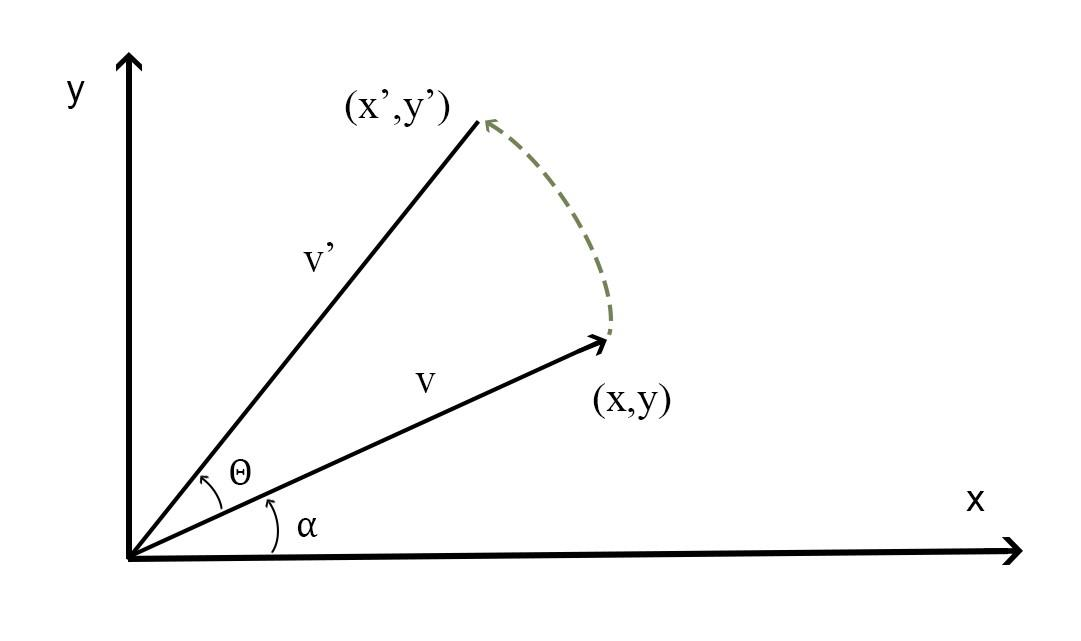
\includegraphics[width=0.60\textwidth]{Pictures/TLfig20.jpg}
    \caption{Transformación de rotación }
    \label{TLfig20}
\end{figure}

\bigskip

\begin{example}
\label{Simetria}
En $\mathbb{R}^3$, consideramos el subespacio $V_1$ correspondiente al  plano $xy$. Si $B= \left\{\vec{e}_1,\vec{e}_2,\vec{e}_3\right\}$ es la base canónica, y $S$ la transformación lineal que  para cada vector $\vec{v}$ da el vector  simétrico con respecto al plano $xy$, como se muestra en la Figura \ref{TLfig30},  se tiene  que  

$$ S(\vec{e}_1)=\vec{e}_1, \quad S(\vec{e}_2)=\vec{e}_2, \quad S(\vec{e}_3)= - \vec{e}_3.$$

Por lo tanto su matriz con respecto a  la base canónica es

$$S=\left(\begin{array}{ccc} 1 & 0 &  0\\
0 &  1  &  0\\
0 &  0  &  -1
\end{array}\right)$$
\end{example}
\begin{figure}
    \centering
    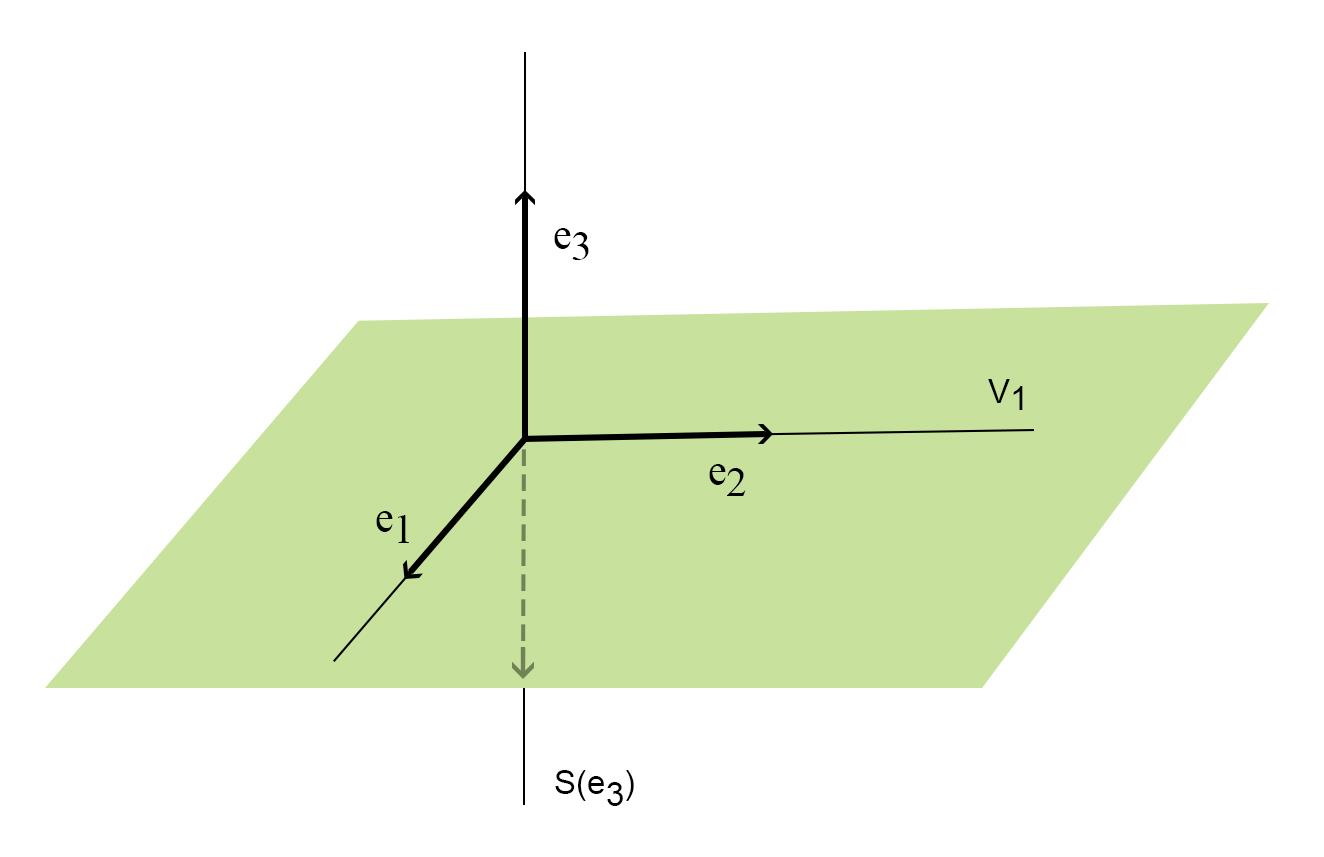
\includegraphics[width=0.90\textwidth]{Pictures/TLfig30.jpg}
    \caption{Simetria con respecto al plano $xy$ }
    \label{TLfig30}
\end{figure}
%(agregar figura pág 256 EH)




\begin{remark}
$\\$
Si se quiere  hallar la matriz que corresponde a la transformación lineal que a cada vector le hace corresponder el vector   simétrico  con respecto a un plano cualquiera, es conveniente   hallar  una base del plano ${ \vec{u}_1, \vec{u}_2}$ y un vector $\vec{u}_3 $ perpendicular.  Así, en la base $\{ \vec{u}_1, \vec{u}_2, \vec{u}_3\} $, la matriz de la simetría con respecto al plano es la misma  que la matriz del Ejemplo \ref{Simetria}. Una vez obtenida la matriz se realiza el cambio de base a la base deseada.
%\hfill$\blacktriangle$
\end{remark}

\bigskip


\begin{example}
De acuerdo a la corolario anterior, para hallar la matriz correspondiente a la simetría con respecto al plano $x+y+z=0$ (Figura \ref{TLfig300}). se busca una base del plano (como $x=-y-z$, los vectores en el plano son de la forma $(-y-z,y,z)=y(-1,1,0)+z(-1,0,1)$, es decir que  los vectores $\vec{u}_1=( -1,1,0)$  y $\vec{u}_2=( -1,0,1)$ son una base del mismo ). Y un vector perpendicular es  $\vec{u}_3=( 1,1,1)$.
En esa  base $\{ \vec{u}_1, \vec{u}_2, \vec{u}_3\} $ la matriz de la simetría con respecto al plano $x+y+z=0$ es, 
entonces,  

$$\left(\begin{array}{ccc} 1 & 0 &  0\\
0 &  1  &  0\\
0 &  0  &  -1
\end{array}\right)$$
\end{example}

\bigskip

\begin{figure}
    \centering
    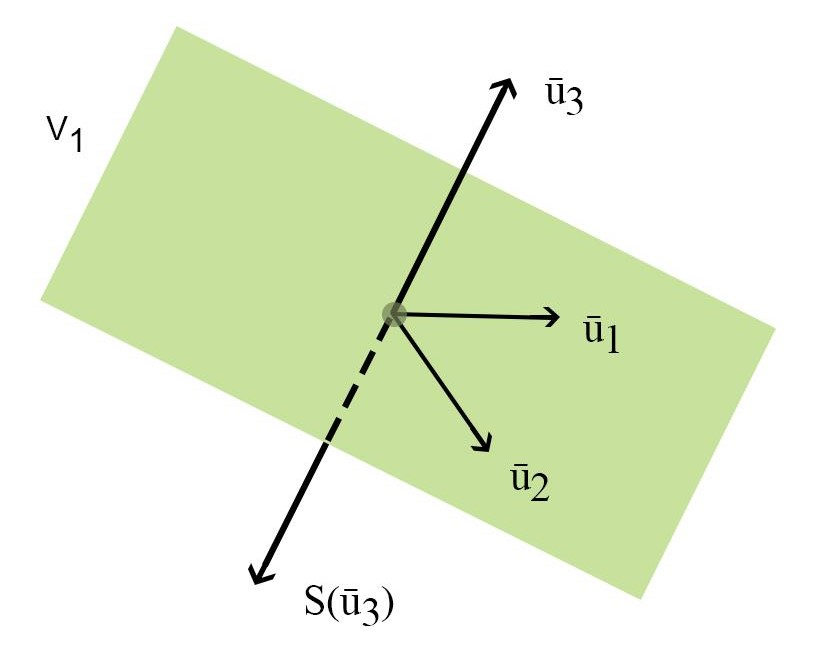
\includegraphics[width=0.65\textwidth]{Pictures/TLfig40.jpg}
    \caption{Simetría respecto al plano $x+y+z=0$ }
    \label{TLfig300}
\end{figure}

\bigskip

\bigskip

Si en los espacios vectoriales $V$ y $W$, de dimensiones finitas $n$ y $m$, respectivamente, se fijan bases, existe una correspondencia biunívoca entre las transformaciones lineales de $V$ en $W$ y el conjunto de las matrices $K^{m \times n}$ (de orden $m \times n$) sobre el cuerpo $K$. Puesto que el conjunto $K^{m \times n}$, posee una estructura de espacio vectorial, también  tiene esa estructura el conjunto de todas las transformaciones lineales entre dos espacios vectoriales sobre el mismo cuerpo $K$. A ese espacio vectorial se lo  denomina $L(V,W)$.


\bigskip

%Las  dos operaciones que le dan estructura de espacio vectorial son:





%Si $T$ y $T ^\prime$ son elementos de $L(V,W)$, definimos la suma mediante

%$$(T+ T ^\prime)(\vec{v})=T(\vec{v})+T^ \prime(\vec{v})~~ para ~todo ~ \vec{v}\in V$$

%Si $T$ es un elemento de $L(V,W)$ y $c$ es un elemento de $K$, se define la multiplicación de $c$ por $T$ mediante

%$$(cT)(\vec{v})=c(T(\vec{v}))~~ para ~todo ~ \vec{v}\in V$$



%Las operaciones recién definidas tienen ciertas propiedades que coinciden con las enumeradas para matrices, y se resumen en el teorema a %continuación:
\bigskip


\bigskip


\begin{corollary}
\label{TEO2}
Sean $V$ y $W$ dos espacios vectoriales sobre un mismo cuerpo $K$; el conjunto $L(V,W)$ de las aplicaciones lineales entre $V$ y $W$, es un espacio vectorial sobre el cuerpo $K$. 

\begin{proof}
\begin{itemize}
\item
Suma. 

Dadas $T_1$ y $T_2$ $ \in  L(V,W)$, se define $T_1+T_2$, $T_1+T_2: V \rightarrow W$  como 
$$ (T_1+T_2)(\vec{v})=  T_1(\vec{v})  +T_2(\vec{v}) \qquad \forall  \vec{v}\in V $$

Veamos que $T_1+T_2$ es una transformación lineal



\begin{itemize}
\item $(T_1+T_2)(\vec{v} + \vec{w} ) = T_1(\vec{v} + \vec{w} )  +  T_2(\vec{v} + \vec{w} )$

$= T_1(\vec{v}) +T_1( \vec{w} )  +  T_2(\vec{v} )+ T_2(\vec{w} )$

$=(T_1+T_2)(\vec{v})     + (T_1+T_2) (\vec{w})$

\bigskip

\bigskip

\item 
$ (T_1+T_2)( \alpha \vec{v})=  T_1( \alpha \vec{v}) + T_2( \alpha \vec{v}) $ 

$=  \alpha T_1( \vec{v}) + \alpha T_2( \vec{v}) $

$= \alpha (T_1( \vec{v}) +  T_2( \vec{v})) = \alpha (T_1 +  T_2)( \vec{v}) $
\end{itemize}

\bigskip

\bigskip

\item
Producto por escalares. 

Dada $T \in L(V,W)$ y $\alpha \in K$, se define  $(\alpha T)$, $(\alpha T): V \rightarrow W$ como 

$$ (\alpha T)(\vec{v})=  \alpha T ( \vec{v}) $$


Veamos que $(\alpha T)$ es una transformación lineal

\bigskip

\begin{itemize}
\item $(\alpha T)(\vec{v} + \vec{w} ) = \alpha (T(\vec{v} + \vec{w} ))$

$= \alpha (T(\vec{v}) + T(\vec{w} ))=  \alpha T(\vec{v}) + \alpha T(\vec{w} )    $

$=(\alpha T)(\vec{v}) + (\alpha T)(\vec{w} )$


\bigskip

\item 
$ (\alpha T)( \beta  \vec{v})=  \alpha (T( \beta  \vec{v})) $ 

$= \alpha (  \beta   T(  \vec{v})) =  (\alpha  \beta)   T(  \vec{v})  $

$= \beta (\alpha T(  \vec{v}))=  \beta (\alpha T)(  \vec{v})  $
\end{itemize}


\end{itemize}

\end{proof}
\end{corollary}



\bigskip

\bigskip

Como toda transformación lineal puede representarse mediante una matriz y recíprocamente, se tiene el siguiente resultado:


\bigskip

\bigskip

\begin{corollary}
\label{TEO3}

Sean $V$ y $W$ espacios vectoriales de dimensiones $n$ y $m$, respectivamente, entonces, el espacio vectorial de las transformaciones lineales del espacio vectorial  $V$ al espacio vectorial $W$, $L(V,W)$,  tiene dimensión $m\times n$.



\begin{proof}
 Se puede ver   en el libro de  E. Hernández \cite{hernandez}. En ella se construye una base de $L(V,W)$. También puede demostrarse  a partir de la correspon-\ dencia biyectiva entre el espacio vectorial de las matrices $K^{m \times n}$ (de dimensión $m \times n$) y  $L(V,W)$.

\end{proof}

\end{corollary}




\begin{remark}
\begin{itemize}
\item
Si $V$ y $W$ coinciden escribimos $L(V)$ en lugar de $L(V,V)$.

\item


La matriz de la aplicación lineal \textit{suma} coincide con la suma de las matrices de cada una de las aplicaciones y la matriz de la aplicación lineal $cT$ coincide con el producto de la matriz $T$ por el escalar $c$. Si llamamos $M(T)$ a la matriz de la aplicación lineal $T$, esto se escribe 

$$M(T+ T ^\prime) = M(T)+M(T ^\prime) \quad \text{y} \quad  M(cT) = cM(T),~ ~ c\in K$$ 
\end{itemize}
%\hfill$\blacktriangle$
\end{remark}


\bigskip

\bigskip

Se verá a continuación que la composición de funciones usual puede realizarse entre dos transformaciones lineales y el resultado es otra transformación lineal.\index{Composición de transformaciones lineales }


\bigskip


\begin{theorem}
\label{Prop342}


Sean $V$, $W$ y $X$ espacios vectoriales sobre el cuerpo $K$. Sean $T\in L(V,W)$ y $T ^\prime\in L(W,X)$. Entonces 

$$ T ^\prime \circ T  \in L(V,X)$$

\begin{proof}

Sean $\vec{v}_1,\vec{v}_2  \in V      $, entonces

\bigskip

$(T ^\prime \circ T )( \vec{v}_1 + \vec{v}_2)= T ^\prime ( T ( \vec{v}_1+ T(\vec{v}_2))= T ^\prime ( T ( \vec{v}_1) )+  T ^\prime (  T(\vec{v}_2)) $

\bigskip

$= (T ^\prime \circ T )( \vec{v}_1)+  (T ^\prime \circ T )( \vec{v}_2) $

Análogamente,

\bigskip


$(T ^\prime \circ T )( \alpha \vec{v})= T ^\prime ( T ( \alpha \vec{v})) = T ^\prime (\alpha T (  \vec{v}))= \alpha  (T ^\prime  \circ T )( \alpha \vec{v})    $
\end{proof}
\end{theorem} 

\bigskip


\begin{theorem}
 Si los espacios $V$, $W$ y $X$ tienen dimensión finita y si denotamos por $M(T)$, $M(T ^\prime)$ y $M(T ^\prime o T)$ las matrices de $T$, $T ^\prime$ y $T ^\prime o T $, respectivamente, con respecto a las bases de antemano fijadas, se tiene el siguiente resultado:

$$M(T ^\prime o T)= M(T ^\prime)M(T)$$

%{\textbf{NOTA:}}  Se puede ver la demostración en el Eugenio Hernández, pág. 261.

\begin{proof}
\begin{equation}
\label{Tej}
T(\vec{e}_j)=\sum_{i=1}^{m}a_{ij}\vec{f}_i,~~ j=1,2 \cdots,n
\end{equation}
donde $a_{ij}$ son los elementos de la matriz $M(T)$.

\bigskip

Sean $\left\{\vec{e}_1,\vec{e}_2,\cdots, \vec{e}_n\right\}$, $\left\{\vec{f}_1,\vec{f}_2,\cdots, \vec{f}_m\right\}$  y $\left\{\vec{g}_1,\vec{g}_2,\cdots, \vec{g}_p\right\}$  bases  de $V$, $W$ y $X$, respectivamente. 
En la $i$-ésima columna de la matriz   $M(T ^\prime o T)$    están las coordenadas del vector $(T ^\prime o T)(\vec{e}_i)$ con respecto a la base $g_k$.

\begin{eqnarray*}
T ^\prime (T(\vec{e}_i))&= &T ^\prime ( \sum_{j=1}^{m}a_{ji}\vec{f}_j)\\
&= &\sum_{j=1}^{m}a_{ji} T ^\prime ( \vec{f}_j)\\
&= &\sum_{j=1}^{m}a_{ji} \sum_{k=1}^{p}b_{kj}  \vec{g}_k\\
&= &\sum_{k=1}^{p}\sum_{j=1}^{m}b_{kj} a_{ji} \vec{g}_k
\end{eqnarray*}
\bigskip
\noindent
donde $b_{ij}$ son los elementos de la matriz $M(T ^\prime)$.

Esto prueba que $  \sum_{j=1}^{m}b_{kj} a_{ji}$ es el elemento que ocupa el lugar $(k,i)$ de la matriz $ M(T ^\prime o T)$ y este valor coincide con el elemento $(k,i)$ del producto de las matrices $M(T ^\prime)$ y $M(T)$.

\end{proof}
\end{theorem} 

\bigskip

\begin{remark}
El resultado anterior se generaliza para el caso de una sucesión de tranformaciones lineales, $T_i$, $i=1, \cdots k$ aplicadas a un vector $\Vec{v}$. Se tendrá entonces que resulta equivalente a aplicar a $\Vec{v}$ una única matriz $T$ tal que   $$M(T)= M(T_k)M(T_{k-1}) \cdots M(T_{2}) M(T_{1})  .$$
%\hfill$\blacktriangle$
\end{remark}

\bigskip

\section{Transformaciones lineales inyectivas y suryectivas.}\index{Transformación lineal inyectiva}\index{Transformación lineal suryectiva}
\label{TLIYS}

Sean $V$ y $W$ dos espacios vectoriales sobre el mismo cuerpo $K$ y $T$ una aplicación lineal de de $V$ en $W$. Recordamos que $T$ es inyectiva si 
$T(\vec{x})=T(\vec{y})$ implica $\vec{x}=\vec{y}$ y $T$ es suryectiva si para todo $\vec{y} \in W$ existe $\vec{x} \in V$ tal que $T(\vec{x})=\vec{y}$ (o equivalentemente $T(V)=W$, donde $T(V)$ denota la imagen de $V$ mediante $T$). Finalmente recordamos que $T$ es \textit{biyectiva} si es a la vez inyectiva y suryectiva.


\begin{remark}\index{Monomorfismo}\index{Epimorfismo}\index{Isomorfismo}
$\\$
En el caso de tranformaciones lineales cada uno de los tipos anteriores recibe un nombre especial: una aplicación lineal \textit{inyectiva} recibe el nombre de \textit{monomorfismo}; si es \textit{suryectiva }se le da el nombre de \textit{epimorfismo}; finalmente si la aplicación es \textit{biyectiva} se dice que es un \textit{isomorfismo}.
%\hfill$\blacktriangle$
\end{remark}




Encontraremos ahora condiciones sencillas que sirvan para determinar si una aplicación lineal es de cualquiera de los tipos anteriores. Comenzaremos con las aplicaciones inyectivas, y para ello necesitamos definir el concepto de \textit{núcleo }de una aplicación lineal.

\section{Núcleo e imagen  de una  transformación  lineal.}
\label{Núcleo e Imagen}

\bigskip

\begin{definition}\label{Nucleo}\index{Núcleo  de una transformación lineal}
Dada una aplicación lineal $T: V \rightarrow W$, 
 definimos el \textit{núcleo} de $T$, que se denota por $N(T)$ (o $Ker(T)$, del inglés \textit{kernel} significa núcleo), como el conjunto de todos los $\vec{v} \in V$ tal que $T(\vec{v})=\vec{0}$, es decir 


$$N(T)=\left\{\vec{v}~ \in V, / T(\vec{v})=\vec{0} \right\}$$

\end{definition}

\bigskip

\bigskip

El subconjunto $N(T)$ nunca es vacío, ya que $\vec{0} \in N(T)$ y esto se deduce de que $T(\vec{0})=\vec{0}$ como ya fue demostrado. Se tiene además, el siguiente resultado:

\bigskip


\bigskip

\begin{theorem}
\label{Prop343}


Si $T: V \rightarrow W$ es una aplicación lineal entre espacios vectoriales, $N(T)$ es un subespacio vectorial de $V$.

\begin{proof}

Esta propiedad  es consecuencia de la Proposición \ref{Prop33}. Por definición $N(T)$ es la preimagen de $\vec{0}_W$ que es un subespacio de $W$.
\end{proof}
\end{theorem} 



%\begin{thm}
%\label{Prop344}

%Si $T: V \rightarrow W$ es una aplicación lineal entre espacios vectoriales. La imagen mediante $T$ de cualquier subespacio vectorial de %$V$ es un subespacio vectorial de $W$.

%\begin{proof}
%\end{proof}
%\end{thm} 

%(ver Prop. 4 pág. 44)

\bigskip


\begin{theorem}
\label{Prop345}

Una aplicación lineal  $T: V \rightarrow W$ es inyectiva si y sólo si  $N(T)=\left\{\vec{0} \right\}$.



\begin{proof}
\begin{itemize}
\item
Si $T$ es inyectiva se tiene que $ T(\Vec{v})=T(\Vec{v}^{\prime})$ implica que $\vec{v}=\Vec{v}^{\prime}$. Si $\exists ~ \Vec{v} ~\in N(T)$  tal que  $T(\vec{v})=\vec{0}  $ como $T(\vec{0})=\vec{0}$ resulta $\vec{v}=\vec{0}$.
\item
Para ver que $T$ es inyectiva suponemos $\exists $ $\vec{v}$ y $\vec{v}^{\prime}$, tales que $ T(\vec{v})=T(\vec{v}^{\prime})$.

Por ser $T$ una transformación lineal $T(\vec{v})=T(\vec{v}^{\prime})= T( 
  \vec{v}-\vec{v}^{\prime})$, y si $T( \vec{v}-\vec{v}^{\prime})= \vec{0} $, entonces,  $\vec{v}-\vec{v}^{\prime} ~ \in ~ N(T)$. 
  
  Como $N(T)=\left\{\vec{0} \right\}$, se tiene que $\vec{v}=\Vec{v}^{\prime}$ y por lo tanto $T$ es inyectiva.
 
  
\end{itemize}
\end{proof}
\end{theorem} 

\bigskip

\begin{example}
Para la proyección ortogonal $P$   de la Figura \ref{figproyxy} (Ejemplo \ref{proyxy}), $$N(P) = \{(x,y,z) \in \mathbb{R}^3 \text{  tales que  } P(x,y,z)=(x,y,0)=(0,0,0) \}.$$ O sea $N(P)= \{ (0,0,z), ~z \in \mathbb{R} \}$ o sea todo el eje $z$. Por  la Proposición \ref{Prop345}, se tiene que  $P$  no es inyectiva (intuitivamente se ve que muchos vectores de 
$\mathbb{R}^3$  dan el mismo vector al proyectarlos  sobre el plano $xy$).
Además, se tiene que  las dimensiones  de $N(P)$ y de la $Im(P)$ son $1$ y $2$, respectivamente, suman $3$, que es la dimensión de $\mathbb{R}^3$. 
\end{example}

\bigskip

\begin{remark}
Si bien las soluciones de un sistema $A\vec{X}=\vec{b}, ~  \vec{b} \neq \vec{0}$  son un subconjunto pero no un subespacio de    $\mathbb{R}^n$ (ver Observación 
 \textcolor{blue}{{\fontfamily{qcr}\selectfont{i}}} en \ref{SHSNH}), toda solución puede expresarse de la forma $\vec{X}= \vec{X}_{NH} + \vec{X}_{H}$, donde  $\vec{X}_{NH}$ es solución de $A\vec{X}=\vec{b}$ mientras que  $\vec{X}_{H} \in Nul(A)$.
Esto sale porque si $\vec{X}_{NH}$ es solución de $A\vec{X}=\vec{b}$, $A(\vec{X}_{NH}+\vec{X}_{H})=  A\vec{X}_{NH}+ A\vec{X}_{H}=   \vec{b}+ \vec{0}= \vec{b} $ y si $\vec{X}$ es otra solución de $A\vec{X}=\vec{b}$, entonces $A(\vec{X}- \vec{X}_{NH})= A\vec{X}- A\vec{X}_{NH}=\vec{b}-\vec{b}=\vec{0} $, de donde $\vec{X}- \vec{X}_{NH}  \in Nul(A)$ y por lo tanto $\vec{X}=  \vec{X}_{NH} +\vec{X}_{H} $.

\bigskip

Como ejemplo se deja al lector verificar que la solución del sistema no homogéneo
\begin{equation} 
\left\{ \begin{array} {ccccl} \nonumber
                    x + y + w&\ =&1     \\
                     2x+3y+z+2w &\ = &1  
                    \end{array}
           \right.
\end{equation}

\bigskip
\noindent
es $\vec{X}=  \vec{X}_{NH} +\vec{X}_{H}= (2,-1,0,0)+ \alpha (1,-1,1,0) + \beta (-1,0,0,1) $ con $\alpha$ y $\beta$ $ \in \mathbb{R}$.
\hfill$\blacktriangle$
\end{remark}

\bigskip

\bigskip


Como se demostró en la Proposición \ref{Prop32}, la imagen de una transformación lineal $T$ es un subespacio. En el teorema que sigue se enuncia la relación que existe entre las dimensiones  del núcleo de $T$,  de la imagen de $T$ y la dimensión de $V$:

\bigskip



\begin{corollary}
    \label{Prop346}

Sean $V$ y $W$ dos espacios vectoriales de los cuales $V$ es de dimensión finita y  $T: V \rightarrow W$ es  una aplicación lineal. Entonces

$$ dim(N(T))+dim(Im(T))=dim(V).$$


\begin{proof}
Sea  $n=dim(V)$ y $k=dim(N(T))$,  

\bigskip
\noindent
si $k=n$, entonces $T$ es la aplicación nula y la $dim(Im(T))=0$. Por lo tanto el teorema vale.

\bigskip

Si $k=0$, entonces $T$ es un monomorfismo. Si $B$ es una base de $V$, $T(V)$ es base de la $Im(T)$. Luego la $dim(Im(T))=dim(V)$ y el teorema vale.

\bigskip

Supongamos que $0<k<n$ y sea $ \left\{\vec{v}_1,\vec{v}_2,\cdots, \vec{v}_k\right\}$  una base de $N(T)$. Sean $\vec{v}_{k+1},\vec{v}_{k+2},\cdots, \vec{v}_n$ tales que $ \left\{\vec{v}_1,\vec{v}_2,\cdots, \vec{v}_k, \vec{v}_{k+1},\vec{v}_{k+2},\cdots, \vec{v}_n    \right\}$ es una base de $V$.

\bigskip

Veamos que $ \left\{T(\vec{v}_{k+1}),T(\vec{v}_{k+2}),\cdots, T(\vec{v}_n )   \right\}$  es una base de $Im(T)$. 

\bigskip

En ese caso se tendrá que $dim(N(T))+dim(Im(T))=k + (n-k) = n= dim(V)$.

\bigskip

\begin{itemize}
    \item 
    Si $\vec{w}\in Im(T)$, $ \quad \exists \quad \vec{v} \in V $ tal que $T( \vec{v}) = \vec{w}$. 
    
    Como $\vec{v}= \sum_{j=1}^n  c_j \vec{v}_j $,  $\vec{w}=T(\vec{v})= \sum_{j=1}^n  c_j T(\vec{v}_j )= \sum_{j=k+1}^n  c_j T(\vec{v}_j )$,   ya que $ \left\{\vec{v}_1,\vec{v}_2,\cdots, \vec{v}_k\right\}$  es una base de $N(T)$. 
    
    Entonces, 
    $ \left\{T(\vec{v}_{k+1}),T(\vec{v}_{k+2}),\cdots, T(\vec{v}_n )   \right\}$  es un sistema de genera-\ dores de $Im(T)$.
    
    
   \bigskip 
    
    \item 
    Para ser si en un conjunto linealmente independiente, supongamos 
    
    $ \sum_{j=k+1}^n  c_j T(\vec{v}_j ) = \vec{0}=    T( \sum_{j=k+1}^n   c_j \vec{v}_j )    $. Entonces,
    
    $ \sum_{j=k+1}^n   c_j \vec{v}_j \in ~ N(T) $.  Como $ \left\{\vec{v}_1,\vec{v}_2,\cdots, \vec{v}_k\right\}$ es una base de $N(T)$, existen escalares $c_1, c_2, \cdots, c_k$ tales que 
    
    \bigskip
    
    $ \sum_{j=k+1}^n   c_j \vec{v}_j =   \sum_{j=1}^k   c_j \vec{v}_j  $

     \bigskip
\noindent
    que puede reescribirse
    
    \bigskip
    
    $    \sum_{j=1}^k  (- c_j)  \vec{v}_j + \sum_{j=k+1}^n   c_j \vec{v}_j = 0$
    
    
    \bigskip
    
Se tiene que $c_i=0$, $ \forall  ~ 1 \le i \le n$, 

por ser $ \left\{\vec{v}_1,\vec{v}_2,\cdots, \vec{v}_k, \vec{v}_{k+1},\vec{v}_{k+2},\cdots, \vec{v}_n    \right\}$  una base de $V$. En parti-\ cular $c_i=0$, $ \forall  ~  k+1 \le i \le n$. Luego $ \left\{T(\vec{v}_{k+1}),T(\vec{v}_{k+2}),\cdots, T(\vec{v}_n )   \right\}$ es un conjunto linealmente independiente.   
\end{itemize}
\end{proof}
\end{corollary}
\bigskip

\begin{example}
Se  verificará el teorema anterior para la transformación lineal $T:\mathbb{R}^5 \rightarrow \mathbb{R}^3 $, dada por $T ((z_1,z_2, \cdots, z_5)) = A (z_1,z_2, \cdots, z_5)^T$, donde $A$ es la matriz (ver Observación 
 \textcolor{blue}{{\fontfamily{qcr}\selectfont{i}}} al final de  la Sección \ref{AyT}).





$$A= \left(   \begin{array}{ccccc} 1 & 1 & 1 & 1 & 1 \\ 0 & 1 & 0 & -1 & 1 \\ 1 & 0 & 1 & 2 & 0 \end{array} \right )$$

En primer lugar, se resuelve el sistema homogéneo utilizando eliminación gaussiana (con la matriz ampliada):


   $$\left(   \begin{array}{cccccc} 1 & 1 & 1 & 1 & 1 & 0 \\ 0 & 1 & 0 & -1 & 1 & 0 \\ 1 & 0 & 1 & 2 & 0 & 0\end{array} \right )  \rightarrow  \left(   \begin{array}{cccccc} 1 & 1 & 1 & 1 & 1 & 0 \\ 0 & 1 & 0 & -1 & 1 & 0\\ 0 & -1 & 0 & 1 & -1 & 0\end{array} \right )\rightarrow  
   
   \rightarrow \left(   \begin{array}{cccccc} \underline{1} & 1 & 1 & 1 & 1 & 0 \\ 0 &\underline{1} & 0 & -1 & 1 & 0\\ 0 & 0 & 0 & 0 & 0 & 0\end{array} \right )$$
   
\bigskip
   
Al quedar solo dos pivotes, hay $2$ variables dependientes y $n-2=3$ variables independientes. Se tiene que dim(N(T))=3.


\bigskip

Para estudiar cuál es el subespacio que corresponde a la imagen de $T$, se debe hallar el subespacio de $\mathbb{R}^3$ que generan las columnas. Puede repetirse la eliminación anterior con término independiente $(x,y,z)$. 

\bigskip

$$\left(   \begin{array}{cccccc} 1 & 1 & 1 & 1 & 1 & x \\ 0 & 1 & 0 & -1 & 1 & y \\ 1 & 0 & 1 & 2 & 0 & z\end{array} \right )  \rightarrow  \left(   \begin{array}{cccccc} 1 & 1 & 1 & 1 & 1 & x \\ 0 & 1 & 0 & -1 & 1 & y\\ 0 & -1 & 0 & 1 & -1 & z-x\end{array} \right )\rightarrow  

\rightarrow \left(   \begin{array}{cccccc} \underline{1} & 1 & 1 & 1 & 1 & x \\ 0 & \underline{1} & 0 & -1 & 1 & y\\ 0 & 0 & 0 & 0 & 0 & z-x+y\end{array} \right )$$


\bigskip
Se tiene, entonces que $Im(T)= \left\{ (x,y,z)=( x,y, x-y) \right\}$, es el plano por el origen $z=x-y$, y

 \bigskip
 
$$dim(N(T))+dim(Im(T))= 3 + 2 = 5= dim(V),$$

\bigskip

\noindent
ya que $V= \mathbb{R}^5$.
 \end{example}

Para deducir algunas consecuencias del Teorema \ref{Prop346} es necesario hacer uso del concepto de \textit{rango}.\index{Rango de una matriz}

\bigskip

Sea $T$ una aplicación entre los espacios vectoriales $V$ y $W$, ambos de dimensión finita, $m$ y $n$ respectivamente. Sea $A$ la matriz de la aplicación lineal en dos bases cualesquiera de $V$ y $W$. Para encontrar el núcleo de $T$, $N(T)$, es necesario resolver el sistema homogéneo $A{\vec{\textbf{x}}}=\vec{0}$ (como se hizo en el ejemplo anterior). 

Si $r(A)$ es el rango  de la matriz $A$, se  obtienen, $r(A)$ soluciones dependien-\ tes y  $n-r(A)$ soluciones linealmente independientes. Es decir que

$$dim(N(T))=dim(V)-r(A)$$
\noindent
y comparando con el Teorema \ref{Prop346}, se tiene que 

$$dim(Im(T))=r(A)$$


\bigskip



Puesto que la dimensión de la $Im(T)$ no depende de las bases que se elijan en $V$ y $W$, de la igualdad anterior se deduce que  las matrices de la aplicación $T$ en cualquier base tienen el mismo rango.

\bigskip

Como consecuencia de lo anterior, es posible definir el \textit{rango de una transformación lineal} $T$, que escribiremos $r(T)$ como el rango de una cualquiera de sus
representaciones matriciales,  y resumir los resultados anteriores en el Corolario que sigue:


\bigskip

\textcolor{orange}{\textbf{Corolario}}
Sean $V$ y $W$ dos espacios vectoriales de los cuales $V$ es de dimensión finita y $T$ una transformación lineal, $T: V \rightarrow W$. Entonces


\begin{enumerate}

\item 

$T$ es inyectiva sí y sólo sí $r(T)=dim(V)$.


\item 

$T$ es suryectiva sí y sólo sí $r(T)=dim(W)$.


\end{enumerate}
%\end{remark}
%{\hfill{\tiny\ensuremath{\blacksquare}}

\bigskip


\bigskip
Por último se estudian las aplicaciones lineales entre espacios vectoriales de igual dimensión que son biyectivas. Se conocen como isomorfismos.
Supongamos que $V$ y $W$ son espacios vectoriales de dimensión finita, y que $T$ es un isomorfismo entre ellos. Del Corolario anterior deducimos que 

$$dim(V)=r(T)=dim(W)$$


\bigskip

Otras consecuencias  de  resultados anteriores se resumen en el teorema que sigue.

\bigskip

\bigskip

\begin{corollary}
\label{Prop347}





Sean $V$ y $W$ espacios vectoriales  de dimensión finita $n$  y  sea $T: V \rightarrow W$ es  una aplicación lineal. Las siguientes condiciones son equivalentes:

\bigskip

\begin{enumerate}

\item  $T$ es biyectiva


\item  $T$ es inyectiva

\item $N(T)=\left\{\vec{0} \right\}$

\item  $T$ es suryectiva

\item  El rango de $T$ es $n$

\end{enumerate}

\bigskip
%manual de latex pag30
\begin{proof}
Entre $2$, $3$, $4$ y $5$ se tienen las equivalencias siguientes:


\[ 
\begin{array}{ccc}
2 & \stk{Prop. \ref{Prop345}} & 3 \\
\Updownarrow{Corolario} &   &  \\
5  & \stk{Corolario}  & 4
\end{array}
\]
Además, $1  \rightarrow 2$ porque toda transformación biyectiva es inyectiva. Como $2$ y $4$ son equivalentes en este contexto y ambas implican $1$, se tiene que también  $2 \rightarrow 1$, y queda demostrado.
%$\stk{Prop. \ref{Prop345}}$
\end{proof}
\end{corollary} 


\bigskip


\bigskip

%\textbf{Isomorfismo}


Decimos que dos espacios vectoriales cualesquiera son \textit{isomorfos} si podemos encontrar un isomorfismo entre ellos. Para que esto ocurra entre espacios vectoriales de dimensión finita ya vimos que ambos han de tener la misma dimensión. El recíproco también es cierto.

\bigskip

\bigskip

\begin{corollary}
\label{Prop348}

Dado cualquier número natural $n$, todos los espacios vectoriales de dimensión $n$ sobre un mismo cuerpo son isomorfos.

\bigskip


\begin{proof}Sean $V$ y $W$ dos espacios vectoriales de dimensión $n$ con bases $\left\{\vec{e}_1,\vec{e}_2,\cdots, \vec{e}_n\right\}$ y $\left\{\vec{e}^{\prime}_1,\vec{e}^{\prime}_2,\cdots, \vec{e}^{\prime}_n\right\}$ respectivamente. 
Existe una transfor-\ mación lineal $T_1$, $T_1: V \rightarrow K^n$ definida de la forma siguiente:

\bigskip

Si $\Vec{v}=\sum_{i=1}^n \alpha_i \vec{e}_i$, $$T_1(\Vec{v})=(\alpha_1, \alpha_2, \cdots , \alpha_n) $$


\bigskip

Es decir que la transformación da el vector con las coordenadas de $\Vec{v}$.
Se demuestra fácilmente (y se deja al lector) que esta transformación es lineal, inyectiva y suryectiva. Al ser biyectiva, existe también su transformación inversa  (Proposición \ref{Prop347}).
Utilizando este isomorfismo de un espacio vectorial $V$ con $K^n$, se tiene que dos espacios cualesquiera de la misma dimensión sos isomorfos. Para encontrar la transformación entre $V$ y $W$ hay que  componer la transformación  $T_1$ entre V y  $K^n$ con la transformación $T_2$ entre   $K^n$ y el espacio vectorial $W$, $T_2: K^n  \rightarrow  W$.
Esta última está dada por

$$T_2(\alpha_1, \alpha_2, \cdots , \alpha_n) = \sum_{i=1}^n \alpha_i \vec{e}^{\prime}_i.$$

\bigskip

El isomorfismo entre $V$ y $W$ está dado por la transformación $$(T_2 \circ T_1)(\Vec{v})=T_2(T_1(\Vec{v}))=\Vec{w}= \sum_{i=1}^n \alpha_i \vec{e}^{\prime}_i  .$$
\end{proof}
\end{corollary} 

\bigskip

\begin{example}
 Aplicando el Teorema anterior, el isomorfismo entre $P_{\mathbb{R}}^{(2)}[t]$ y  $\mathbb{R}^3$  está dado por 
$$T( a_0 1+ a_1 t + a_2 t^2)= (a_0, a_1, a_2)^t,$$
mientras que el isomorfismo entre   $\mathbb{R}^3$ y las matrices simétricas  de $\mathbb{R}^{2\times2 }$  está dado por:
$$T(x,y,z)= \left(   \begin{array}{cc} x & y \\ y & z   \end{array} \right ).$$

\bigskip

Se consideraron  las bases canónicas de  $\mathbb{R}^3$, de $P_{\mathbb{R}}^{(2)}[t]$ y  de las matrices simétricas de $\mathbb{R}^{2\times2 }$,  espacios vectoriales de dimensión $3$. 
Se deja al lector la verificación de estos resultados.
\end{example}

\bigskip

\begin{remark}
Si $T$ es un isomorfismo entre dos espacios vectoriales $V$ y $W$ de dimensión $n$, por el Teorema \ref{Prop347}, su rango es $n$, y por lo tanto la matriz $M(T)$ de $T$ en cualesquiera bases de $V$ y $W$ es \textit{invertible}. Además, la inversa de $M(T)$ es la matriz de la aplicación inversa de $T$.
%\hfill$\blacktriangle$
\end{remark}


\bigskip

\begin{example}
%Ejemplos
%hojitas 15 y
Sean $V$ y $W$  dos espacios vectoriales de funciones,   de dimensión infinita:

 \bigskip
 
 $V=\{ f \in C^1[0,1] / f(0)=0 \}$ y $W=C[0,1] $.

 \bigskip
 
Sea la transformación 

\bigskip
 
 $D: V  \rightarrow W$ dada por $D(f)= f^{\prime}$. $D$ es una transformación lineal (En el Ejemplo \ref{ejderi} se vió para polinomios en $P_R^{(n)}[x]$) .
 \begin{itemize}
\item
$D$ es monomorfismo

Supongamos $D(f)=D(g)$, entonces $f^{\prime}= g^{\prime}$ o, en forma equivalente $(f-g)^{\prime}=0$. Entonces $f(x)-g(x)=cte$. Como $f(0)=g(0)=0$, se tiene que la $cte=0$, por lo tanto $f=g$. 
\item
$D$ es epimorfismo

Sea $g \in W$ y sea 

\[
f(x)=\int_0^x g(t)dt.
\]
Entonces, por el Teorema Fundamental del cálculo, $f \in C^1[0,1]$  y $f^{\prime}=g(x)$,  $ \forall  x \in [0,1]$.
Más aún, como \[
\int_0^0 g(t)dt=0, 
\]
\noindent
se tiene que 
$f(0)=0$. Por lo tanto, $\forall g \in W,  ~ \exists f \in V $  tal que $Df=g$. O sea $D$ es epimorfismo.
\end{itemize}
Resulta, entonces, que $V$ y $W$ son espacios isomorfos.
\end{example}

\bigskip

\index{González, Gabriela}
\begin{parchment}[Gabriela González] {Gabriela González es una física, investigadora y profesora argentina. Nació en 1965. Fue portavoz y coordinó durante seis años un equipo de mil especialistas, que trabajó en las detecciones de ondas gravitacionales efectuadas desde el proyecto LIGO (Ondas Gravitacionales con Interferómetro Láser, por sus siglas en inglés). En febrero de 2016 fue una de los cuatro científicos de LIGO que anunciaron la primera observación ondulatoria gravitacional, detectada en septiembre de 2015. Egresada de la Universidad Nacional de Córdoba y actual profesora en el departamento de física y astronomía de la Universidad de Louisiana, fue reconocida en 2016 como una de los diez científicos más destacados del mundo por la revista académica Nature. Además, a partir de 2018 forma parte de la Academia de Ciencias de Estados Unidos, institución de máximo prestigio internacional.  \cite{GabG} }
\end{parchment}


\bigskip

\section{Geometría de las transformaciones  lineales  de $\mathbb{R}^2$ en  $\mathbb{R}^2$   }
Se verán en esta sección algunas propiedades geométricas de las transformaciones lineales en el plano.
Dada la matriz 

$$A=\left(   \begin{array}{cc} a & b \\ c & d   \end{array} \right )$$
\noindent
la transformación $L: \mathbb{R}^2  \rightarrow \mathbb{R}^2$ dada por $L((x,y))=A (x,y)^t$ es $$L  \left( \left(  \begin{array}{c} x  \\ y  \end{array}    \right) \right )=\left(   \begin{array}{c} a x + by  \\ cx +  d y  \end{array} \right )$$ .
\begin{example}
 En la Figura \ref{TLfig50} se muestra la transformación que a cada vector le hace corresponder el simétrico respecto del eje $y$.
 \index{Reflexión}

 $$L  \left( \left(  \begin{array}{c} x  \\ y  \end{array}    \right) \right )= \left(   \begin{array}{cc} -1 & 0 \\ 0 & 1   \end{array} \right ) \left( \begin{array}{c} x  \\ y  \end{array} \right )     =\left(   \begin{array}{c} - x   \\ y  \end{array} \right )$$ .
\end{example}


\begin{figure}
    \centering
    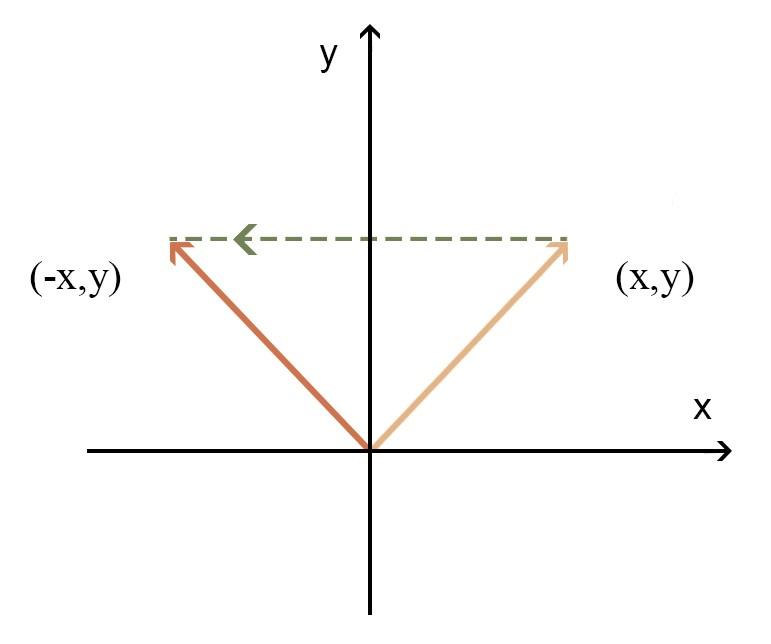
\includegraphics[width=0.50\textwidth]{Pictures/fig.13.jpg}
    \caption{Transformación de simetría (o reflexión) respecto del eje $y$ }
    \label{TLfig50}
\end{figure}

\begin{example}
 En la Figura \ref{TLfig60} se muestra la transformación que a cada vector le hace corrresponder el simétrico respecto del eje $x$

 $$L  \left( \left(  \begin{array}{c} x  \\ y  \end{array}    \right) \right )= \left(   \begin{array}{cc} 1 & 0 \\ 0 & -1   \end{array} \right )\left( \begin{array}{c} x  \\ y  \end{array} \right )      =\left(   \begin{array}{c} x   \\ -y  \end{array} \right )$$ .
\end{example}

\begin{figure}
    \centering
    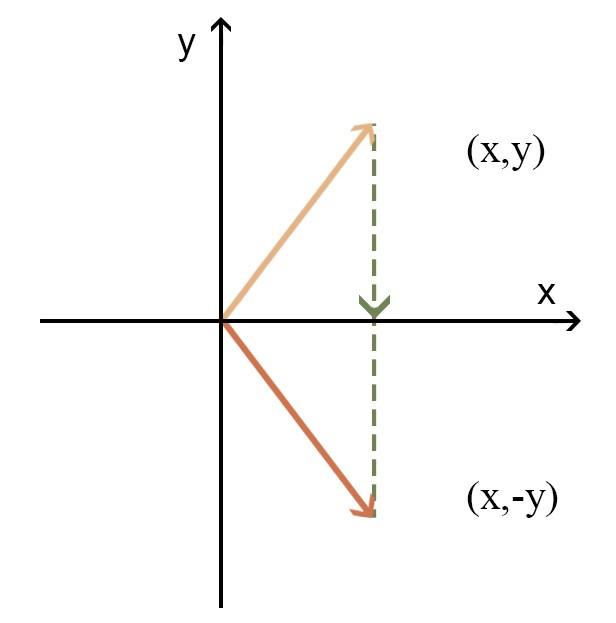
\includegraphics[width=0.50\textwidth]{Pictures/fig.14.jpg}
    \caption{Transformación de simetría respecto del eje $x$ }
    \label{TLfig60}
\end{figure}


\begin{example}
\label{proyejex}
 En la Figura \ref{fig36} se muestra la transformación que a cada vector le hace su proyección ortogonal sobre el eje $x$:

 $$L  \left( \left(  \begin{array}{c} x  \\ y  \end{array}    \right) \right )= \left(   \begin{array}{cc} 0 & 1 \\ 1 & 0   \end{array} \right ) \left( \begin{array}{c} x  \\ y  \end{array} \right )    =\left(   \begin{array}{c} x   \\ 0  \end{array} \right ).$$ 
\end{example}


\begin{figure}
    \centering
    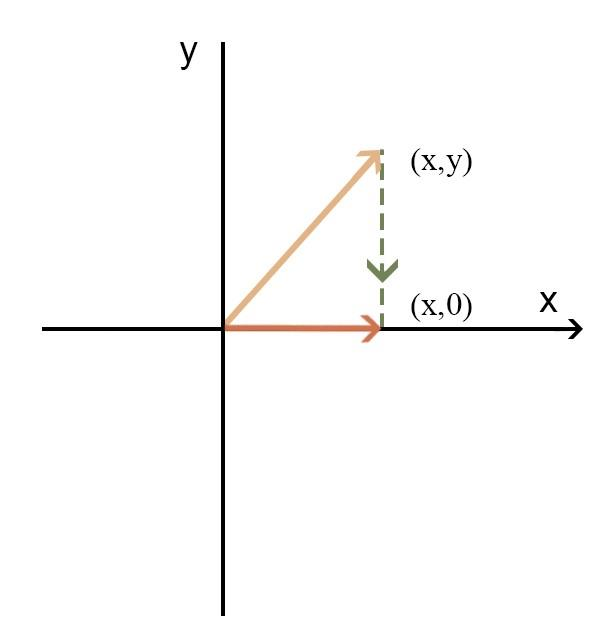
\includegraphics[width=0.50\textwidth]{Pictures/fig.36.jpg}
    \caption{Proyección ortogonal sobre el eje $x$ }
    \label{fig36}
\end{figure}



\begin{example}
\index{Reflexión}
 En la Figura \ref{TLfig77} se muestra la transformación que a cada vector le hace su reflexión  respecto de la recta  $y=x$:

 $$L  \left( \left(  \begin{array}{c} x  \\ y  \end{array}    \right) \right )= \left(   \begin{array}{cc} 0 & 1 \\ 1 & 0   \end{array} \right ) \left( \begin{array}{c} x  \\ y  \end{array} \right )     =\left(   \begin{array}{c} y   \\ x  \end{array} \right )$$ .
\end{example}
\begin{figure}
    \centering
    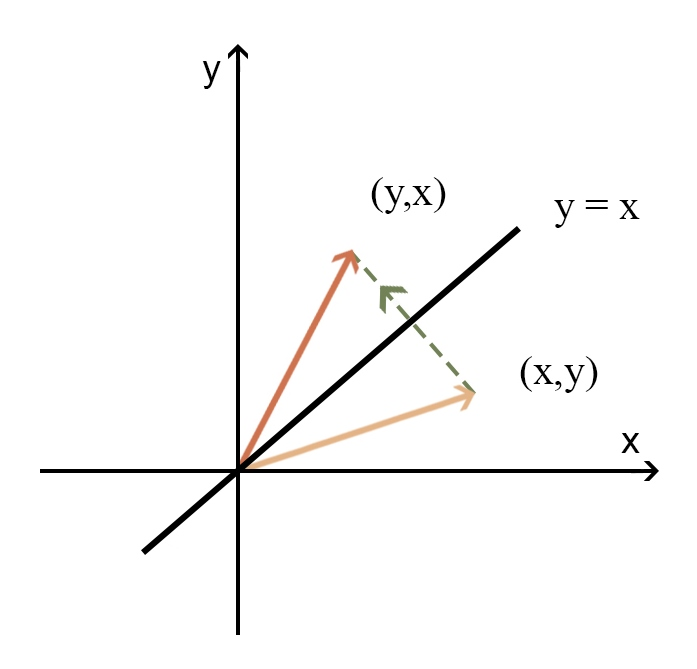
\includegraphics[width=0.50\textwidth]{Pictures/fig.17.jpg}
    \caption{Transformación de reflexión respecto de la recta $y=x$ }
    \label{TLfig77}
\end{figure}

\bigskip

\begin{remark}
 Otras  transformaciones se obtienen al multiplicar una de las  coordenadas por una constante $k$. Así el efecto es comprimir o dilatar en esa dirección, dependiendo si $k < 1$ o $k > 1$. También están las transformaciones llamadas de \textit{trasquillado}, dadas por matrices de la forma:

 $$L  \left( \left( \begin{array}{c} x  \\ y  \end{array}    \right) \right )= \left(   \begin{array}{cc} 1 & k \\ 0 &  0   \end{array} \right ) \left( \begin{array}{c} x  \\ y  \end{array} \right )     =\left(   \begin{array}{c} x+ky   \\ y  \end{array} \right ).$$
 %\hfill$\blacktriangle$
\end{remark}

Estos casos se analizarán en los ejercicios propuestos.


\begin{figure}
    \centering
    %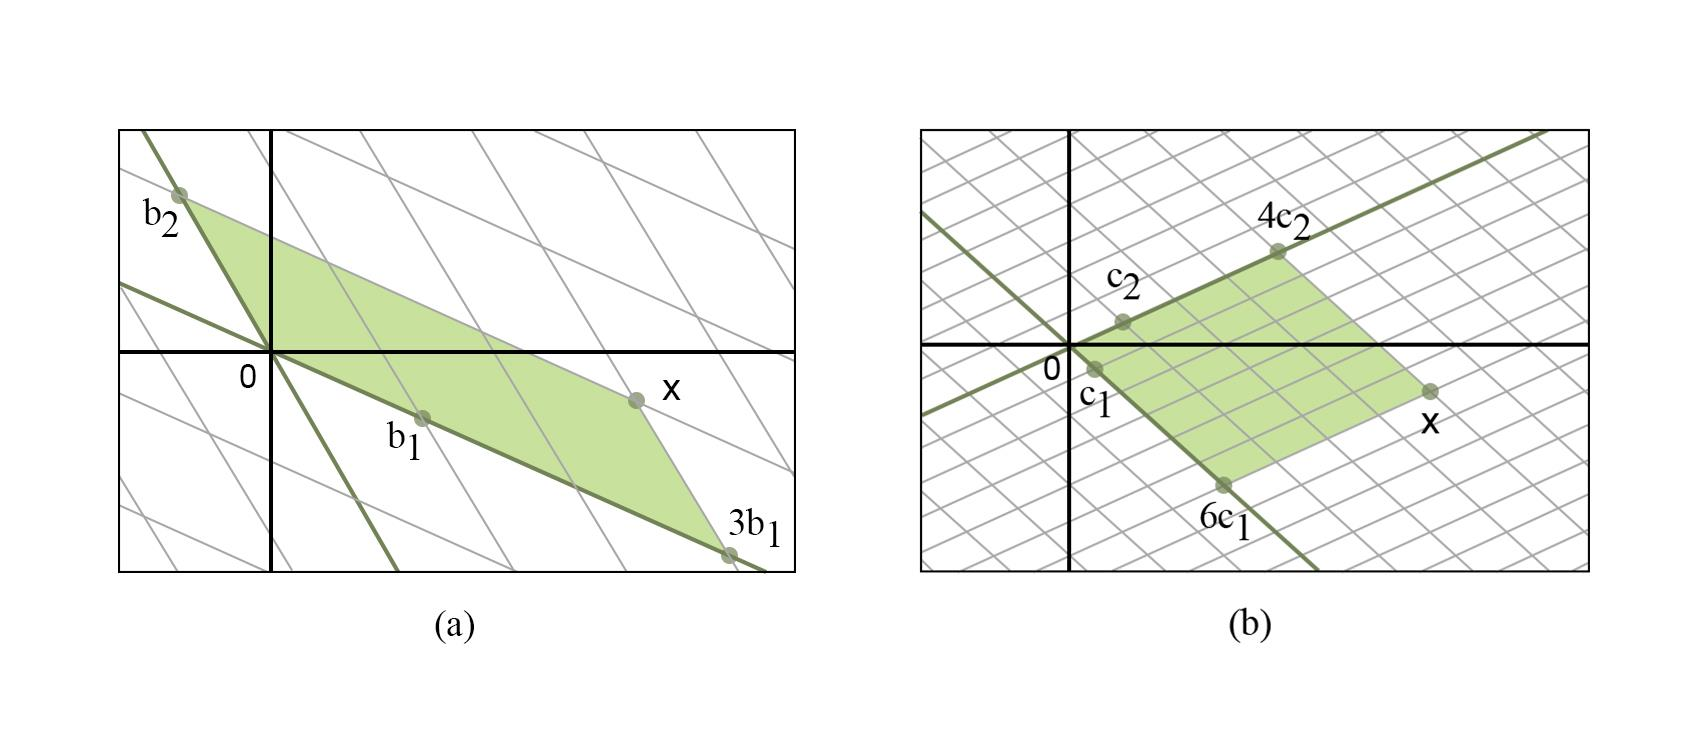
\includegraphics[width=0.90\textwidth]{Pictures/TLfig80.jpg}
    %\caption{Transformación de simetría respecto de la recta $y=x$ }
    \label{TLfig70}
\end{figure}


%\end{document}

\section{Cambio  de base para transformaciones  lineales}
 \label{cbaseTL}

Sean $V$ y $W$ dos espacios vectoriales sobre el mismo cuerpo $K$ de dimensiones $n$ y $m$, respectivamente. Sea $T$ una transformación lineal de $V$ en $W$ con matriz 

$$T=(a_{i,j})_{i,j=1,n}$$

\bigskip

\noindent
con respecto a las bases $B= \left\{\vec{e}_1,\vec{e}_2,\cdots, \vec{e}_n\right\}$  y $\bar{B}= \left\{\vec{f}_1,\vec{f}_2,\cdots, \vec{f}_n\right\}$   de $V$ y $W$, respectivamente. 

\bigskip


Si queremos conocer la matriz $T^{\prime} =(a_{i,j})_{i,j=1,n}$ de la misma aplicación $T$ respecto a dos nuevas bases  $B^{\prime}= \left\{\vec{e}^{\prime}_1,\vec{e}^{\prime}_2,\cdots, \vec{e}^{\prime}_n\right\}$  y $\bar{B^{\prime}}= \left\{\vec{f}^{\prime}_1,\vec{f}^{\prime}_2,\cdots, \vec{f}^{\prime}_n\right\}$   de $V$ y $W$, respectivamente, es necesario realizar los cambios de base adecuados en los espacios vectoriales  inicial y final, $V$ y $W$.



\bigskip


\noindent
Para seguir el razonamiento, veamos el diagrama siguiente

 %\begin{center}
 %    {\framebox{
 %         \parbox {8.5cm}{\begin{center} {$B= \left\{\vec{e}_1,\vec{e}_2,\cdots, \vec{e}_n\right\}$ \end{center}}}}   
%nd{center}
%
%newcommand{\stk}[1]{\stackrel{#1}
%{\longrightarrow}}
%\newcommand{\cT}{\mathcal{T}}
%\newcommand{\dwn}[1]{
%{\scriptstyle #1}\downarrow}
%\[
%\begin{array}{ccc}
%U       & \stk{G}  & \cT  U\\
%\dwn{\phi}  &      &  \dwn{\cT\phi}\\
%$B^{\prime}= \left\{\vec{e^{\prime}}_1,\vec{e}_2,\cdots, \vec{e}_n\right\}$  & \stk{\cT\phi\circ G\circ\phi}     &  \cT\phi(\cT U)
%\end{array}
%\]

\newcommand{\stk}[1]{\stackrel{#1}
{\Longrightarrow}}
\newcommand{\cT}{\mathcal{T}}
\newcommand{\dwn}[1]{
{\scriptstyle #1}\Uparrow}
\[
%\begin{center}
\begin{array}{ccc}
      V           & y=T(x)         &    W        \\\\
B= \left\{\vec{e}_1,\vec{e}_2,\cdots, \vec{e}_n\right\}    & \stk{a_{i,j}}  &  \bar{B}= \left\{\vec{f}_1,\vec{f}_2,\cdots, \vec{f}_n\right\} \\
\dwn{C}  &      &  \dwn{D} \\
B^{\prime}= \left\{\vec{e}^{\prime}_1,\vec{e}^{\prime}_2,\cdots, \vec{e}^{\prime}_n\right\}  & \stk{a^{\prime}_{i,j}}    &  \bar{B^{\prime}}= \left\{\vec{f}^{\prime}_1,\vec{f}^{\prime}_2,\cdots, \vec{f}^{\prime}_n\right\}
\end{array}
%\end{center}
\]

\bigskip

\bigskip

En el diagrama

\bigskip

\begin{itemize}
\item

$a_{ij}$ son los elementos de  la matriz de la transformación $T$ tomando la base $ B$ en $V$ y la base  $\bar{B}$ en $W$   
\item
$a^{\prime}_{ij}$ son los elementos de  la matriz de la transformación $T$ tomando la base $ B^{\prime}$ en $V$ y la base  $\bar{B}^{\prime}$ en $W$   \item
 $C$ y $D$ son las matrices del cambio de base de $B^{\prime}$ a $B$ y de $\bar{B^{\prime}}$ a $\bar{B}$, respectivamente.
\end{itemize}

\bigskip


Se tiene que $\vec{x}\in V$ puede escribirse de dos formas 

\bigskip

$$ x_1\vec{e}_1+x_2\vec{e}_2+\cdots +x_n\vec{e}_n = x^{\prime}_1\vec{e}^{\prime}_1+x^{\prime}_2\vec{e}^{\prime}_2+\cdots +x^{\prime}_n\vec{e}^{\prime}_n $$


\bigskip
e   $\vec{y}=T(\vec{x})$ también


\bigskip

$$ y_1\vec{f}_1+y_2\vec{f}_2+\cdots +y_n\vec{f}_n = y^{\prime}_1\vec{f}^{\prime}_1+y^{\prime}_2\vec{f}^{\prime}_2+\cdots +y^{\prime}_n\vec{f}^{\prime}_n $$


\bigskip

\bigskip

\bigskip

En primer lugar, se tiene que, 

\bigskip

\begin{eqnarray}
\label{yTx}
\left(\begin{array}{c} y_{1} \\ y_{2}  
\\  y_3 \\ \cdots \\ y_{n} 
\end{array} \right)=T\left(\begin{array}{c} x_{1} \\ x_{2}  
\\  x_3 \\ \cdots \\ x_{n} 
\end{array} \right)
\end{eqnarray}

\bigskip

\noindent
y de acuerdo a los cambios de base en un mismo espacio vectorial que se estudiaron antes, 


$$\left(\begin{array}{c} x_{1} \\ x_{2}  
\\  x_3 \\ \cdots \\ x_{n} 
\end{array} \right)=C\left(\begin{array}{c} x^{\prime}_{1} \\ x^{\prime}_{2}  
\\  x^{\prime}_3 \\ \cdots \\ x^{\prime}_{n} 
\end{array} \right)~~~~~~~~\left(\begin{array}{c} y_{1} \\ y_{2}  
\\  y_3 \\ \cdots \\ y_{n} 
\end{array} \right)=D\left(\begin{array}{c} y^{\prime}_{1} \\ y^{\prime}_{2}  
\\  y^{\prime}_3 \\ \cdots \\ y^{\prime}_{n} 
\end{array} \right)$$
\bigskip
mientras que, considerando las bases ${B^{\prime}}$ y   $\bar{B^{\prime}}$, se tiene que, 
\bigskip
\begin{eqnarray}
\label{yTpx}
\left(\begin{array}{c} y^{\prime}_{1} \\ y^{\prime}_{2}  
\\  y^{\prime}_3 \\ \cdots \\ y^{\prime}_{n} 
\end{array} \right)=T^{\prime}\left(\begin{array}{c} x^{\prime}_{1} \\ x^{\prime}_{2}  
\\  x^{\prime}_3 \\ \cdots \\ x^{\prime}_{n} 
\end{array} \right)
\end{eqnarray}
\bigskip



Sustituyendo en (\ref{yTx}),  se obtiene, 


$$D\left(\begin{array}{c} y^{\prime}_{1} \\ y^{\prime}_{2}  
\\  y^{\prime}_3 \\ \cdots \\ y^{\prime}_{n} 
\end{array} \right)=TC\left(\begin{array}{c} x^{\prime}_{1} \\ x^{\prime}_{2}  
\\  x^{\prime}_3 \\ \cdots \\ x^{\prime}_{n} 
\end{array} \right)$$

\bigskip

\noindent
y como $D$ es una matriz de cambio de base, tiene inversa, por lo tanto


$$\left(\begin{array}{c} y^{\prime}_{1} \\ y^{\prime}_{2}  
\\  y^{\prime}_3 \\ \cdots \\ y^{\prime}_{n} 
\end{array} \right)=D^{-1}TC\left(\begin{array}{c} x^{\prime}_{1} \\ x^{\prime}_{2}  
\\  x^{\prime}_3 \\ \cdots \\ x^{\prime}_{n} 
\end{array} \right)$$

\bigskip

\noindent
Comparando esta expresión con (\ref{yTx}) se obtiene, finalmente que 

$$T^{\prime}= D^{-1}TC,$$

\bigskip

\noindent
y es posible  calcular la matriz $T^{\prime}$ de la aplicación  $T$ con respecto a las bases $B^{\prime}$ y $\bar{B^{\prime}}$, conocidas la matriz $T$ de la misma aplicación con respecto a las bases $\bar{B}$ y $\bar{B^{\prime}}$ y las matrices $C$ y $D$ del cambio de base $B^{\prime}$ a $B$ y de $\bar{B^{\prime}}$ a $\bar{B}$, respectivamente.

\newpage

\begin{remark}\index{Matrices equivalentes} \index{Matrices semejantes}
\label{Obssemejanza}
\begin{itemize}
\item
Cuando entre dos matrices $T$ y  $T^{\prime}$ se tiene la relación 
$T^{\prime}= D^{-1}TC$, se dice que las matrices $T$ y  $T^{\prime}$ son \textit{equivalentes}  (  $D$ y $C$ son matrices invertibles). Y si  las matrices $D$ y $C$ coinciden, se dice que las matrices $T$ y  $T^{\prime}$ son  \textit{semejantes}.

\item
En muchos casos los espacios inicial $V$  y final $W$  de una transformación lineal coinciden, y se anota $T \in L(V)$. 

\item
Cuando  $B$ y $\bar{B}$ coinciden y $B^{\prime}$ y  $\bar{B^{\prime}}$ coinciden, la fórmula del cambio de base es más sencilla. Si $T$ es la matriz de la aplicación $T\in L(V)$ con respecto a la base $B$ de $V$, la matriz $T^{\prime}$ de la misma aplicación con respecto a una base $B^{\prime}$ de $V$  está dada por 


$$T^{\prime}=C^{-1}TC.$$
\noindent
donde $C$ es la matriz del cambio de base de $B^{\prime}$ a $B$.
Al tener esta relación entre las matrices,  por lo anterior, $T$ y  $T^{\prime}$ son \textit{semejantes}. 

\bigskip

\item

 Si $T^{\prime}=C^{-1}TC$, $Det(T^{\prime})=Det(T)$, ya que 
 \bigskip
 
 $Det(T^{\prime})= Det(C^{-1}TC)= Det(C)^{-1}Det(T).Det(C) \\ = Det(C^{-1}C)Det(T)= Det(I)Det(T)=Det(T)$.
 

\end{itemize}

% ejemplo hojita 15 y problema 6.5
\end{remark}
\bigskip

\bigskip


\begin{example}
\label{ejemplo217}

Si $B$ es la base canónica, $B^{\prime}=\{ (1,2), (2,3) \}$ y  

$$(T)_{B}= \left(   \begin{array}{cc} 6 & -2 \\ 6 &  -1   \end{array} \right )$$

se tiene que 
 $$(T)_{B^{\prime}}= \left(   \begin{array}{cc} 1 & 2 \\ 2 &  3   \end{array} \right )^{-1}\left(   \begin{array}{cc} 6 & -2 \\ 6 &  -1   \end{array} \right ) \left(   \begin{array}{cc} 1 & 2 \\ 2 &  3   \end{array} \right )   = \left(   \begin{array}{cc} 2 & 0 \\ 0 &  3   \end{array} \right )$$.
\end{example}
%\hfill$\blacktriangle$


\bigskip

\section{Espacio dual de un espacio Vectorial.}\index{Espacio dual}


Dado un espacio vectorial $V$ sobre un cuerpo $K$, podemos considerar el conjunto $L(V,K)$ de todas las transformaciones lineales de $V$ en el espacio vectorial  $K$ (de dimensión  $1$ sobre $K$). 

\bigskip


Este espacio vectorial es un caso particular del estudiado anteriormente ($L(V,W)$), y el Teorema \ref{TEO2} de la sección nos permite concluir que $L(V,K)$ es un espacio vectorial sobre $K$. Este espacio vectorial recibe el nombre de \textit{espacio dual} del espacio vectorial $V$  y para indicarlo se utiliza comúnmente el símbolo $V^*$, en lugar de $L(V,K)$. En otras palabras, $V^*$ es el espacio vectorial de todas las aplicaciones lineales de $V$ en $K$, también llamados funcionales lineales..



\bigskip



Los elementos de $V^*$ son transformaciones lineales. Si $V$ es un espacio vectorial de dimensión finita $n$, del  Teorema \ref{TEO3} se deduce que es espacio dual $V^*$  tiene dimensión $n$. El teorema que sigue exhibe una base $B^{*}$ asociada de manera única  y natural a una base $B$ de $V$. La demostración del  Teorema \ref{TEO3}, más general, fue citada. Se presenta a continuación la demostración para este caso particular.

\bigskip

\bigskip


\begin{corollary}
\label{basedual}
Sea $V$ un espacio vectorial de dimensión finita $n$ y  $B= \left\{\vec{e}_1,\vec{e}_2,\cdots, \vec{e}_n\right\}$ una base de  $V$. Existe una única base 

$$B^*= \left\{\varphi_1,\varphi_2,\cdots,\varphi_n\right\}$$
de $V^*$ tal que $\varphi_i(\vec{e}_i)=1$ para todo $i=1, \cdots,n$,   y $\varphi_j(\vec{e}_i)=0$  si $i\neq j$. 
Es decir, los elementos de la base dual de  $B$ satisfacen 
 $$\varphi_j(\vec{e}_i)= \delta_{ij}, \qquad j,i= 1,2, \cdots, n  $$
 
 
La base $B^*$  se denomina \textit{base dual} de $B$.



\bigskip

\begin{proof}
Para $ \vec{v}= \sum_{j=1}^n   v_j \vec{e}_j$,  definimos los funcionales  $\varphi_j$, $j=1,2, \cdots, n$ de la forma siguiente, 
$$ \varphi_j( \vec{v})=v_j  $$
\noindent
es decir, da la coordenada $j$-ésima.

\bigskip 


\begin{itemize}
\item
$\varphi_j  \in V^* $  y satisface $\varphi_j(\vec{e}_i)= \delta_{ij}$

\item
 ¿$\left\{\varphi_1,\varphi_2,\cdots, \varphi_n \right\}$ son linealmente independientes ?
 
 \bigskip
 
 Si $ \sum_{j=1}^n  c_j \varphi_j = \vec{0}   $,  ¿ Se cumple que $c_j = 0, \quad \forall j$ ?
 
\bigskip 

Notar que el término $\vec{0}$ del miembro derecho de la igualdad  es la aplicación nula (la imagen de $\vec{0}$ es $0 \in K$  $ ~\forall \vec{v} \in V$). Se deberá cumplir  esa igualdad  al evaluar  las transformaciones lineales de ambos lados en cualquier vector $\vec{v}$. En particular si se evaluán en los vectores de la base,
 
 \bigskip 

 
$ \sum_{j=1}^n  c_j \varphi_j( \vec{e}_i)= \vec{0}( \vec{e}_i)=0   $, $ ~\forall i=1,2, \cdots, n$. 

\bigskip 

\noindent
Por lo tanto, $~c_i=0, i=1,2,\cdots, n$, ya que  $ \varphi_j( \vec{e}_i)   $ es no nulo solo cuando $j=i$. De ahí que $B^*$ es un conjunto de aplicaciones linealmente independientes.

\bigskip 

\item
Finalmente, para ver que generan, si $A \in V^*$, 

\bigskip 

$A( \vec{v})=A( \sum_{j=1}^n   v_j \vec{e}_j)= \sum_{j=1}^n A(  v_j \vec{e}_j)$

\bigskip 

$=\sum_{j=1}^n v_j A(\vec{e}_j)= \sum_{j=1}^n \varphi_j( \vec{v}) A(\vec{e}_j)=\sum_{j=1}^n A(\vec{e}_j)\varphi_j( \vec{v})      $.

\bigskip 

Entonces, se tiene la igualdad  $$   A= \sum_{j=1}^n A(\vec{e}_j)\varphi_j  $$
\end{itemize}

\bigskip 

\noindent
y por lo tanto, $B^*=\left\{ \varphi_1,\varphi_2,\cdots,\varphi_n\right\}$ es una base y queda demostrado el teorema.


\end{proof}
%\end{theom} 
\end{corollary}

%{\textbf{NOTA:}}

%La propiedad de $B^*$  se escribe más fácilmente usando la \textit{delta} ($\delta$) de %\textit{Kronecker} que ya se introdujo antes:

%$$E_j(\vec{e}_i)=\delta_{ji}$$

\bigskip

\bigskip

\bigskip

\begin{example}
Se quiere hallar la base dual  $ B^* =\left\{\varphi_1,\varphi_2, \varphi_3\right\} $ de la base canónica $B= \left\{\vec{e}_1,\vec{e}_2, \vec{e}_3\right\}$  de $\mathbb{R}^3$.

La transformación lineal $\varphi_1$ debe satisfacer

\bigskip

$\varphi_1 (\vec{e}_1)=1$, $\varphi_1 (\vec{e}_2)=0$, y $\varphi_1 (\vec{e}_3)=0$,
\noindent
de donde se obtiene, 

\bigskip

$\varphi_1( x_1,x_2,x_3)=\varphi_1( x_1 \vec{e}_1+ x_2 \vec{e}_2 + x_3 \vec{e}_3)=x_1$. 

\bigskip


De manera similar, $\varphi_2( x_1,x_2,x_3)=x_2$ y $\varphi_3( x_1,x_2,x_3)=x_3$. 

\end{example}


\begin{example}
\label{polLag}

Sean $L_i$, $i=1,2,3$, funcionales  sobre $P_\mathbb{R}^{(2)}\left[t\right]$, definidos como  $L_i(p(t))=p(t_i)$  donde los $t_i$ son distintos. 

Son aplicaciones lineales y son linealmente independientes, ya que si $c_1 L_1 + c_2 L_2 + c_3 L_3=\vec{0}$, para todo $p \in P_\mathbb{R}^{(2)}\left[t\right]$, entonces $c_1=c_2=c_3=0$.


 

$V= P_\mathbb{R}^{(2)}\left[t\right]$ tiene dimensión $3$. $L_1$, $L_2$ y $L_3$ $\in V^*$ y entonces,
$\left\{L_1, L_2,  L_3 \right\}$ es una base de $V^*$. (Recordar que $V$ y $V^*$ tienen la misma dimensión).



¿Existe una base $B$  de $V$ para la cual $\left\{L_1, L_2,  L_3 \right\}$ es su base dual, $ B^*$?

Es decir se quieren hallar   $\left\{p_1,p_2, p_3 \right\}$ $\in V$  tales que 

$$L_j(p_i)=\delta_{ji}$$

\bigskip

$p_1(t_1)=1$, $p_1(t_2)=0$, $p_1(t_3)=0$

$p_2(t_1)=0$, $p_2(t_2)=1$, $p_2(t_3)=0$

$p_3(t_1)=0$, $p_3(t_2)=0$, $p_3(t_3)=1$

\bigskip

De donde, 




\[
p_1(t)= \frac{(t-t_2)(t-t_3)}{(t_1-t_2)(t_1-t_3)}
\]



\[p_2(t)= \frac{(t-t_1)(t-t_3)}{(t_2-t_1)(t_2-t_3)}\]



\[p_3(t)= \frac{(t-t_1)(t-t_2)}{(t_3-t_1)(t_3-t_2)}\]

\bigskip







Para cada $p \in V$, 
\bigskip

$p(t)=L_1(p(t))p_1(t) + L_2(p(t)) p_2(t) + L_3(p(t))p_3(t)= p(t_1)p1(t) + p(t_2) p_2(t) + p(t_3) p_3(t) $

\bigskip

$p_1(t),p_2(t), p_3(t)$ son los polinomios de interpolación de Lagrange. Es importante señalar que estos polinomios tienen muchas aplicaciones en aproximación de funciones y en integración numérica.

\bigskip

Es posible, por ejemplo,  expresar el polinomio $p(t)=t^2+1$ como combinación lineal de los funcionales $L_i$ si $t_1=0$, $t_2=1$ y $t_3=-1$.

\[
p_1(t)= \frac{(t-t_2)(t-t_3)}{(t_1-t_2)(t_1-t_3)}=\frac{(t-1)(t+1)}{(-1)(1)}=1-t^2
\]



\[p_2(t)= \frac{(t-t_1)(t-t_3)}{(t_2-t_1)(t_2-t_3)}=\frac{(t)(t+1)}{(1)(2)}=\frac{(t^2+t)}{2}\]



\[p_3(t)= \frac{(t-t_1)(t-t_2)}{(t_3-t_1)(t_3-t_2)}=\frac{(t)(t-1)}{(-1)(-2)}=\frac{(t^2-t)}{2}\]

\bigskip


Como $L_i(p)=p(t_i)$, se tiene que 

\bigskip


$L_1(p)=p(t_1)= p(0)=1$, $~L_2(p)=p(t_2)= p(1)=2$, y $ L_3(p)=p(t_3)= p(-1)=2$.

\bigskip

Finalmente,

\bigskip


$p(t)=L_1p_1(t) + L_2 p_2(t) + L_3p_3(t)= p(t_1)p_1(t) + p(t_2) p_2(t) + p(t_3) p_3(t)$

\bigskip

$p(t)= (1)(1-t^2) + 2 \frac{(t^2+t)}{2} + 2 \frac{(t^2-t)}{2}= t^2+1  $


\bigskip

Esta última es la expresión de $p(t)$ en la base $\left\{p_1,p_2, p_3 \right\}$. Notar que sus coordenadas están dadas por $L_i(p)=p(t_i)$, $i=1,2,3$.

\end{example}
\bigskip

Siempre es  posible hallar la base de $B$ como se hizo en el ejemplo anterior. Asi como toda base de $V$ de dimensión finita tiene una base dual asociada, toda base de $V^*$ es la base dual de una base de $V$. Esta   propiedad importante -de la cual no incluimos la demostración- se enuncia en el teorema a continuación.

\bigskip

\begin{corollary}
\label{basedeV}

Sea $V$ un espacio vectorial de dimensión finita $n$ y  sea $V^*$  su espacio dual.  Sea $B^{\prime}= \left\{\phi_1,\phi_2,\cdots, \phi_n\right\}$ una base de  $V^*$. Existe una única base $B= \left\{\vec{v}_1,\vec{v}_2,\cdots, \vec{v}_n\right\}$ de $V$ que satisface  $B^* = B^{\prime}  $.
\end{corollary}

\bigskip


\textbf{Relación entre las coordenadas en las bases $B$ y $B^*$}
Si $B$ es una base de un espacio vectorial $V$ de dimensión finita y 
$$B^*= \left\{\varphi_1,\varphi_2,\cdots,\varphi_n\right\}$$  es su base dual, es posible calcular fácilmente las coordenadas de un elemento de $V$ usando la base $B^*$ como se realizó al final del  Ejemplo \ref{polLag}. Y recíprocamente es posible hallar las coordenadas  de un elemento de $V^*$ utilizando la base $B$. Esto se muestra en el ejemplo que sigue:

\bigskip

\begin{example}
Si 
$B= \left\{\vec{e}_1,\vec{e}_2\right\}=  \left\{(1,1),(1,-1)\right\}    $ y 


\[B^*= \left\{\varphi_1,\varphi_2\right\}=\left\{\frac{x+y}{2},\frac{x-y}{2}\right\} \]

La relación entre las coordenadas en las bases $B$ y $B^*$ es:

\bigskip

$(5,5)= \alpha (1,1) + \beta  (1,-1)$


\bigskip


$\varphi_1(5,5)= \alpha \varphi_1(1,1) + \beta \varphi_1 (1,-1)=  \alpha$

\bigskip

$\varphi_2(5,5)= \alpha \varphi_2(1,1) + \beta \varphi_2 (1,-1)=  \beta$

\bigskip

ya que $ \varphi_i(\vec{e}_j)= \delta_{ij} $.

\bigskip

Por otro lado, dado un funcional $\varphi(x,y) ~\in V^*$, $\varphi(x,y) = \alpha^* \varphi_1 (x,y) + \beta^*  \varphi_2(x,y)  $

Así, para 

\bigskip
\noindent
\[\varphi(x,y) = 3 x + 5 y = \alpha^* (\frac{x+y}{2}) +\beta^*  (\frac{x-y}{2}) \]



\bigskip

\noindent
sus coordenadas son,  $  \alpha^* =\varphi(1,1)$ y $  \beta^*= \varphi(1,-1) $ 

\bigskip

 Entonces, la relación entre las coordenadas es la siguiente:
 
\bigskip
 
$$\alpha=\varphi_1(5,5)=5 \qquad\beta=\varphi_2(5,5)=0$$


$$\alpha^*= \varphi (1,1)=8  \qquad\beta^* = \varphi(1,-1) =-2$$

\bigskip



\end{example}
\bigskip


Se puede generalizar lo que vimos en el ejemplo anterior. 
%Si $B$ es una base de $V$y $B^*$ su base dual, es posible calcular las coordenadas de un elemento de $V$  en la base %$B$ usando $B^*$, y recíprocamente usando $B$ es fácil obtener las coordenadas en la base $B^*$ de un elemento de $V^*$.

\bigskip

Sean 
$B= \left\{\vec{e}_1,\vec{e}_2,\cdots, \vec{e}_n\right\}$ una base de  $V$  y $B^*= \left\{\varphi_1,\varphi_2,\cdots, \varphi_n\right\}$ una base de  $V^*$.


\bigskip

\begin{itemize}
\item
Dado  $\vec{v} \in V$, $\vec{v}=  \sum_{i=1}^n  \alpha_i \vec{e}_i  $,  $ \alpha_i \in K  $
\begin{equation}
 \label{alphaj}   
 \varphi_j(\vec{v}) = \varphi_j( \sum_{i=1}^n  \alpha_i \vec{e}_i)=  ( \sum_{i=1}^n  \alpha_i \varphi_j(\vec{e}_i))= \alpha_j.
\end{equation}

\bigskip

Luego, 

\bigskip


$ (\vec{v} )_B=   ( \varphi_1( \vec{v} ), \varphi_2( \vec{v} ),  \cdots,   \varphi_n( \vec{v} ) ) $

\bigskip

\item

Dada $\varphi \in  V^* $, $\exists \quad \beta_i \in K   $ tal que  $\varphi=  \sum_{i=1}^n  \beta_i \varphi_i  $

\bigskip

Para cada $j$, $   1 \le j \le n$, 


\begin{equation}
 \label{betaj}   
\varphi(\vec{e}_j )  = (\sum_{i=1}^n  \beta_i \varphi_i) (\vec{e}_j ) = \sum_{i=1}^n  \beta_i \varphi_i (\vec{e}_j )  \beta_j   
\end{equation}
\bigskip

Luego, 

\bigskip

$(\varphi)_{B^*}= ( \varphi(\vec{e}_1 )   ,   \varphi(\vec{e}_2),  \cdots,  \varphi(\vec{e}_n  ))$



\end{itemize}

\bigskip

\begin{remark}
En el Ejemplo \ref{polLag} las coordenadas de $p(t)$ son, de acuerdo a (\ref{alphaj}), $L_i(p(t))=p(t_i)$, $i=1,2,3$.
%\hfill$\blacktriangle$
\end{remark}

\bigskip

\subsubsection{Anulador de un subespacio.}

Existe también relación entre  los subespacios de $V$ con ciertos subespacios de $V^*$. En particular, dado un subespacio $S$ de $V$ si consideramos el conjunto de todas los funcionales  lineales que se anulan en $S$ se prueba  que tiene una estructura de subespacio.

\bigskip

\bigskip

\begin{definition}\index{Anulador de un subespacio}
\noindent
Sea $V$ un espacio vectorial y sea $S$ un subespacio de $V$. Se llama \textit{anulador} al conjunto 
$$S^0=\left\{\varphi~ \in V^*, \varphi(\Vec{s})=0 ~ \forall \Vec{s} \in S\right\}$$
$$=\left\{\varphi~ \in V^*, ~ S \subseteq N(\varphi) \right\}$$
\end{definition}


\bigskip


\begin{theorem} $S^0$ es un subespacio de $V^*$.

% hojita 20


\begin{proof}
\begin{itemize}
\item
$\Vec{0}~ \in ~ S^0 $ (se anula en todo $S$ y $\Vec{0}~ \in ~ S$).
\item
Si $\varphi_1$ y $\varphi_2$ $ ~ \in ~ S^0$, entonces $\varphi_1(\Vec{s})=0$ y  $\varphi_2(\Vec{s})=0$   $\forall~\Vec{s} ~ \in ~ S $, de donde $(\varphi_1 + \varphi_2)(\Vec{s})=\varphi_1(\Vec{s})+\varphi_2(\Vec{s})  =0 $  $\forall~\Vec{s} ~ \in ~ S $. Se tiene,  que 
$\varphi_1 + \varphi_2  \in ~S^0$.
\item
Si $c ~\in ~ K $ y $\varphi_1$ $ \in ~ S^0$, $ (  c \varphi_1)(\Vec{s})=c \varphi_1(\Vec{s})= c 0= 0 $  $\forall~\Vec{s} ~ \in ~ S $. Luego, $  c \varphi_1  \in ~S^0$.
\end{itemize}
\end{proof}
\end{theorem} 

\bigskip


\begin{theorem} 
\label{TeodimS0}
Sea $V$ un espacio vectorial de dimensión $n$ y sea $S$ un subespacio de $V$. Entonces 
$$dim(S)+dim(S^0) = n$$

\bigskip

\begin{proof}
% pag 101 UBA y ejemplo
Sea $\left\{\vec{v}_1,\vec{v}_2,\cdots, \vec{v}_k\right\}$ una base de $S$, y sean $  \vec{v}_{k+1},\vec{v}_{k+2},\cdots, \vec{v}_n\  ~ \in V$  tales que \\ $B=\left\{\vec{v}_1,\vec{v}_2,\cdots, \vec{v}_k,  \vec{v}_{k+1},\cdots, \vec{v}_n \right \}$ sea una base de $V$.

Sea $ B^* =\left\{\varphi_1,\varphi_2,\cdots, \varphi_k, \varphi_{k+1}, \cdots, \varphi_k \right\}  \subset V^*$ la base dual de $B$. Entonces, para cada $k+1 \leq i \leq n$, se tiene que $ \varphi_i(\vec{v}_1)=\varphi_i(\vec{v}_2) =\cdots = \varphi_i(\vec{v}_k)=0 $, y por lo tanto    $\varphi_i $  se anula en todo $S$. Se tiene que   $  \left\{\varphi_{k+1}, \cdots, \varphi_n \right\}$ $  \subseteq  ~S^0$.

  Como $  \left\{\varphi_{k+1}, \cdots, \varphi_n \right\}$ es parte de una base, es un conjunto linealmente independiente. Veamos que es un sistema de generadores de $S^0$ y entonces es base de $S^0$.

\bigskip

  Sea $ \psi  \in ~S^0 $. Como $ B^*$ es una base de $V^*$, existen $  c_1,c_2, \cdots, c_n ~ \in K $ tales que 
$ \psi = \sum^n_{i=1} c_i \varphi_i$. Por la relación entre las coordenadas (\ref{betaj}) se tiene que $  c_i= \psi(\vec{v}_i)=0$. Además, como $ \psi \in ~S^0$ y $\left\{\vec{v}_1,\vec{v}_2,\cdots, \vec{v}_k\right\}$ una base de $S$, $ \psi(\vec{v}_i)=0$ para cada $1 \leq i \leq k$. En consecuencia, $c_i=0$  para $1 \leq i \leq k$, y por lo tanto $ \psi \in \langle \varphi_{k+1}, \cdots, \varphi_n  \rangle $. 

\bigskip

Luego, $  \left\{\varphi_{k+1}, \cdots, \varphi_n \right\}$ es una base de $S^0$ y entonces, $$dim(S^0) = n - k = n-dim(S). $$
\end{proof}
\end{theorem}

\bigskip



\bigskip

\bigskip


\begin{example}
Se quiere hallar el subespacio anulador  $S^0$  para 

$S\langle (1,1,1),(1,2,1)\rangle \subset  \mathbb{R}^3 $.
De acuerdo a la demostración de la Proposición \ref{TeodimS0}, $S^0= \langle \varphi_3 \rangle$. Se completa $S$ para tener una  base de $\mathbb{R}^3$, $B= \left\{\vec{v}_1,\vec{v}_2,\vec{v}_3\right\}= \left\{(1,1,1), (1,2,1),(1,0,0)\right\} $ y luego, a partir de escribir $(x,y,z)$ como combinación lineal de esa base y teniendo en cuenta que  $\varphi_i(\vec{v}_j)=\delta_{ij}$, se obtiene que $\varphi_3(x,y,z)=x-z$.

\end{example}
Veremos  que los sistemas de ecuaciones lineales (como el del Ejemplo \ref{ejsistema}),  pueden estudiarse  desde el punto de vista de los funcionales lineales.

\bigskip


\begin{example}
Sea el sistema lineal homogéneo:


\begin{equation} 
\left\{ \begin{array} {ccl} \nonumber
                    x_1+ x_3 &\ =&0      \\
                     2x_1-x_2+x_3 &\ = &0 \label{ejemplosistdual}
                   \end{array}
           \right.
\end{equation}

%Si se consideran las bases canónicas de $\mathbb{R}^3$ y del dual (ver ejemplo XXX)

%Las ecuaciones pueden escribirse como  2 funcionales $  \varphi_1 $  y $  \varphi_2 $, en términos de la base $E^*$ :

%$$\varphi_1(x_1,x_2,x_3) = E_1 + E_3  $$

%$$\varphi_2(x_1,x_2,x_3) = 2E_1 - E_2 + E_3  $$

\bigskip


Sea $S$ el subespacio de $\mathbb{R}^3$ generado por $\alpha_1=(1,0,1)$, $\alpha_2=(2,-1, 1)$. Entonces el espacio solución es el espacio anulador,  $S^0$.
Es decir,  $~\varphi\in S^0 \Leftrightarrow  \varphi(\alpha_i)=0$, para $i=1,2$.

\bigskip
Resolviendo el sistema homogéneo, se tiene que $S= \langle (-1,-1,1)\rangle$. Para hallar una base de $S^0$, se deben realizar los pasos de la demostración de la Proposición \ref{TeodimS0}:
\begin{itemize}
    \item 
    Se completa la base de $S$ para tener una base de $\mathbb{R}^3$, $B\left\{\vec{v}_1,\vec{v}_2, \vec{v}_3\right\}$, por ejemplo,
    
    $B=\left\{(-1,-1,1),(1,0,0),(0,0 1)\right\} $.
\item
Se halla la base $ B^* = \left\{\varphi_1,\varphi_2, \varphi_3 \right\}$ tal que  $\varphi_j(\vec{v}_i)= \delta_{ij}, \quad i,j= 1,2,3$.
 \item   
La base de $S^0$ está dada por $  \left\{\varphi_{2}, \varphi_3 \right\}= \left\{ x_1-x_2, x_2+x_3 \right\} $.
\end{itemize}
\end{example}




Se verá a continuación cómo se comporta el anulador con la suma y la intersección de subespacios:

\bigskip

\begin{theorem} Sea $V$ un espacio vectorial de dimensión $n$ y sean $S$ y $T$  subespacios de $V$. 


Entonces, 

\bigskip

\begin{enumerate}
\item
$(S+T)^0 = S^{0}\cap T^{0}$  y 

\item

$(S\cap T)^{0}=S^{0} +T^{0}$ 
\end{enumerate}
\bigskip

\begin{proof}
% pag 102 uba

\begin{enumerate}
\item
Sea $ \varphi \in V^*$. Se tiene que $ \varphi \in (S+T)^0$ sí y solo sí $ \varphi(\Vec{s} + \Vec{t})=0$ para todo $\Vec{s} \in S$  y   para todo $\Vec{t} \in T$. Y esto es equivalente a que  $\varphi(\Vec{s})=0$ para todo  $\Vec{s} \in S$  y $\varphi(\Vec{t})=0$  para todo $\Vec{t} \in T$, es decir que  $\varphi \in  S^{0}\cap T^{0}$.

\bigskip

\item
Sea $ \varphi \in  S^{0} +T^{0}$. Entonces $ \varphi= \varphi_S + \varphi_T$, $\varphi_S \in  S^{0} $ y $\varphi_T \in  T^{0} $. Para cada $\Vec{x} \in S\cap T $ se tiene que $ \varphi(\Vec{x})=\varphi_S (\Vec{x})+  \varphi_T(\Vec{x})=0+0=0 $. Luego $  \varphi  \in (S\cap T)^{0}$. Por lo tanto $ S^{0} +T^{0}   \subseteq (S\cap T)^{0} $. Por el Teorema de la dimensión para la suma de subespacios (Proposición \ref{2131}),  teniendo en cuenta que $(S+T)^0 = S^{0}\cap T^{0}$ y la Proposición \ref{TeodimS0},

\begin{eqnarray*}
dim(S^{0} +T^{0})&=&dim(S^{0}) + dim(T^{0}) - dim (S^{0}\cap T^{0})\\
& = & dim(S^{0}) + dim(T^{0}) - dim ((S+T)^0)\\
&=& n-dim(S) + n-dim(T)-(n-dim(S+T))\\
&=& n-(dim(S) + dim(T) - dim(S+T))\\
&=& n-dim(S\cap T)\\
&=& dim((S\cap T)^{0})
\end{eqnarray*}

\bigskip

En consecuencia, $(S\cap T)^{0}=S^{0} +T^{0}$.
\end{enumerate}
\end{proof}
\end{theorem} 


%Pueden estudiarse los sistemas de ecuaciones lineales desde el punto de vista de los funcionales lineales


%\begin{example}

%Sea $W$ el subespacio de $\mathbb{R}^{(5)}$ generado por $\alpha_1=(2,-2,3,4,-1)$, $\alpha_2=(-1,1,2,5,2)$, %$\alpha_3=% %(0,0,-1,-2,3)$, $\alpha_4=(1,-1,2,3,0)$

%\bigskip

%Hallar $W^0$.



%Consideramos



%$A= \left(\begin{array}{ccccc}  2 & -2 &  3 & 4 & -1 \\ -1 & 1 &  2 & 5 & 2    \\     0 & 0 &  -1 & -2 & 3  \\     1 & %-1 &  2 & 3 & 0 
%\end{array}
% \right)$


%Si $\varphi$ es un funcional sobre $\mathbb{R}^{(5)}$, es de la forma 


%$\varphi(x_1,x_2,x_3,x_4,x_5)= c_1 x_1 + c_2 x_2 + c_3 x_3 + c_4 x_4 + c_5 x_5$


%y $\varphi\in W^0 \Leftrightarrow  \varphi(\alpha_i)=0$, para $i=1,2,3,4$

%terminar hojita 21
%\end{example}

\bigskip


\bigskip


\subsubsection{El doble dual}\index{Doble dual}

\bigskip

Como $V^*=L(V,K)$ es un espacio vectorial,  es posible definir su espacio  dual. Entonces $(V^*)^*=L(V^*,K)$. Por las propiedades vistas antes, se tiene que  $dim(V)=dim(V^*)=dim(V^{**})$.
Si $V$ es de dimensión finita, sabemos que los espacios $V$ y $V^*$, al tener la misma dimensión, son isomorfos. Para hallar el isomorfismo se debe hallar una base de $V$ y su base dual. En forma similar, como la dimensión de $V^*$  es igual a la dimensión de $V^{**}$, existe un isomorfismo  entre los espacios $V^*$ y $V^{**}$. En este segundo caso,  el isomorfismo  no requiere la elección de bases, y se dice que es natural. 

\bigskip



%Sea $\vec{v} \in V$. Se tiene una aplicación $L_{\vec{v}}: V^* \rightarrow K$

%$$L_v(\varphi)=\varphi(v)$$


%\textbf{Nota}

%Si $dim(V)<\infty$ y $v\neq \vec{0}$,  entonces $L_{\vec{v}}\neq \vec{0}$ 

%   hojita 24 (ver dem. como ejercicio)

%\bigskip

\begin{theorem}

Sea $V$ un espacio vectorial,  $dim(V)<\infty$ sobre $K$. Para cada vector $v \in V$, se define
$L_v: V^* \rightarrow K$, $L_{\vec{v}}(\varphi)=\varphi(\vec{v})$, $\varphi \in V^*$.


\bigskip

La aplicación 
$\phi:V \rightarrow V^{**}$ que a $\vec{v}$ hace corresponder $L_v(\varphi)$ es un isomorfismo.
%($\varphi(\vec{v})=L_{\vec{v}}$).


\bigskip


Notar que   $L_v$ se aplica a elementos de $V^*$ y debe dar un escalar. La definición indica que, aplicado a $\varphi$ ese escalar es $\varphi(\vec{v})$, de ahí que el nombre de este isomorfismo es la \textit{evaluación}, ya que para cada $\varphi$ da su evaluación en $\vec{v}$,  $\varphi(\vec{v})$.
\begin{proof}
Se deja al lector probar que $L_v$ es una transformación lineal. Como $V$ y $~V^{**}$ tienen la misma dimensión, alcanza con probar que la transforma-\ ción es inyectiva.

\bigskip

Sea $\vec{v} \in N(\phi)$. Entonces $L_{\vec{v}}(\varphi)=0$ para todo $\varphi$ en  $V^*$, o sea 
$\varphi(\vec{v})=0$  para todo $\varphi$ en  $V^*$. El único elemento de $V$ con esta propiedad (da $0$ en cualquier funcional $V^*$), es $\vec{0}$. Es decir que $N(\phi)= \vec{0}$. Así que, $\phi$ es inyectiva, y por lo tanto, es un isomorfismo.


% hojita 23 y 24 poner como ejercicio
\end{proof}
\end{theorem}


\begin{remark}
Si $V$ tiene dimensión infinita la aplicación $\phi:V \rightarrow V^{**}$ sigue siendo inyectiva, pero no suryectiva. Así que no todo espacio de dimensión infinita es isomorfo a su doble dual.
%\hfill$\blacktriangle$
\end{remark}
%\bigskip
%\noindent
%\textbf{Corolario 1}


%Sea $V$ un espacio vectorial,  $dim(V)<\infty$ sobre $K$. Si  $L \in V^*$, existe un único  $\vec{v} \in V$ tal que %$L(\varphi)=\varphi(\vec{v})$ para todo $\varphi \in V^*$.

%\bigskip
%\noindent
%\textbf{Corolario 2}


%Sea $V$ un espacio vectorial,  $dim(V)<\infty$ sobre $K$. Toda base de    $V^*$, es la base dual de alguna base de $V$.

\bigskip

\subsubsection{Aplicación transpuesta}\index{Aplicación transpuesta}

\noindent
Sean $V$ y $W$ dos espacios vectoriales de  $dim<\infty$ sobre $K$. 
Sea $T: V \rightarrow W$ una aplicación lineal. $T$ induce una aplicación lineal  de $W^*$ en $V^*$ que llamaremos \textit{transpuesta }de $T$, 

Si $\phi: W \rightarrow K$,

\bigskip

$$T^t: W^* \rightarrow V^*$$

$$T^t(\varphi)=\phi \circ T$$

$$T^t(\varphi)(\vec v)=\varphi(T(\vec v))$$

\bigskip

Se deja al lector probar que $T^t(\varphi)$ es una transformación lineal.
% hojita 24'

\bigskip


\begin{theorem}

Sean $V$ y $W$ dos espacios vectoriales sobre el mismo cuerpo $K$. Sea $T$ una aplicación lineal de $V$ en $W$, entonces

$$N(T^t)=Im(T)^0$$

\bigskip
Se deja la prueba al lector.
%\noindent
%Si  $V$ y $W$ tienen  $dim<\infty$, entonces $T$ y $T^t$ tienen el mismo rango ($r(T)=r(T^t)$). 





%\begin{proof}
% falta
%\end{proof}
\end{theorem}

\bigskip



\textbf{Relación entre las matrices que representan a una aplicación lineal y su traspuesta}

\bigskip

\noindent
Sean $T: V \rightarrow W$  y  $T^t: W^* \rightarrow V^*$. Y sean $B$ y $B^{\prime}$ bases de $V$ y $W$ respectivamen-\ 
te, y  $B^*$ y $B^{\prime *}$   bases de $ V^*$  y $W^*$, respectivamente.


\bigskip

 Si $A=\left[T\right]_{B ^{\prime},B}$ y $C=\left[T^t\right]_{ B^*  ,B ^{\prime *}}$, entonces $C=A^t$


\bigskip


\begin{example}

 En este ejemplo se muestra la relación  entre las matrices de la transformación $T$ y la  de su aplicación  transpuesta $ T^t$, en el caso   $V=\mathbb{R}^2$, $W=\mathbb{R}^3$, y $T: V \rightarrow W$ definida por 
  $T(x,y)=(2x-y,3x,x-2y)$.
  
  Sean las bases de $V$ y $W$,

\bigskip

$B= \left\{(1,2),(1,3)\right\}$  y $B^{\prime}= \left\{(1,1,1),(1,1,0),(1,0,0)\right\}$, respectivamente.
 
\bigskip



\begin{itemize}
    \item 
    Como
$$T((1,2))=  (0,3,-3)= -3(1,1,1,) + 6(1,1,0) -3(1,0,0,)$$

$$T((1,3))=  (-1,3,-5)= -5(1,1,1,) + 8(1,1,0) -4(1,0,0,)$$
\bigskip

la matriz de $T$ en las bases $B$ y $ B^{\prime}$ es 
$\left(\begin{array}{cc}  -3 & -5  \\ 6 &  8 \\ -3  &  -4
\end{array}
 \right)$

\bigskip

Veamos ahora la matriz correspondiente a la transformación transpuesta $ T^t$, $T^t: W^* \rightarrow V^*$ , definida como $T^t(\varphi)(\vec v)=\varphi(T(\vec v))$ y considerando las bases $B^{\prime *}$  de $W^*$  y $B^*$  de $V^*$.
  \item
 $B^*= \left\{ \varphi_1, \varphi_2 \right\}$ 
 
 \bigskip
 
$(x_1,x_2)= \alpha (1,2) + \beta ( 1,3)$
de donde $\alpha + \beta =x_1$ y $2\alpha + 3\beta =x_2$.

\bigskip

Se resuelve el sistema y resulta 

\bigskip

$\varphi_1(x_1, x_2)= \alpha=3x_1 -x_2$

\bigskip

 $\varphi_2(x_1, x_2)= \beta =x_2 -2 x_1$
 
\bigskip

 \item
 $B^{\prime *}=\left\{ \varphi^{\prime}_1, \varphi^{\prime}_2, \varphi^{\prime}_3 \right\}$ 


\bigskip

Para hallar esta base  se hace lo mismo que para  $B^*$, partiendo de 

\bigskip

$(x_1, x_2,x_3)= \alpha (1,1,1)+   \beta (1,1,0)+  \gamma (1,0,0)$

\bigskip


se aplican $\varphi^{\prime}_i$, $i=1,2,3$, y se obtiene 


\bigskip

$\varphi^{\prime}_1(x_1, x_2,x_3)= \alpha=x_3$

 \bigskip
 
$\varphi^{\prime}_2(x_1, x_2,x_3)= \beta=x_2-x_3$

 \bigskip
 
$\varphi^{\prime}_3(x_1, x_2,x_3)= \gamma=x_1-x_2$

 \bigskip
 
 \item
 
Para obtener  la matriz de $ T^t$ se debe calcular

\bigskip

$ T^t ( \varphi^{\prime}_1)(x_1, x_2,x_3)   = \varphi^{\prime}_1(T(x_1, x_2,x_3)) = x_1-2x_2= -3 \varphi_1 - 5 \varphi_2 $


\bigskip

$ T^t ( \varphi^{\prime}_2)(x_1, x_2,x_3)   = \varphi^{\prime}_2(T(x_1, x_2,x_3)) =  6 \varphi_1 + 8 \varphi_2 $ 


 \bigskip

$ T^t ( \varphi^{\prime}_3)(x_1, x_2,x_3)   = \varphi^{\prime}_3(T(x_1, x_2,x_3)) =  -3 \varphi_1 -4 \varphi_2 $ 


\bigskip

La matriz de $T^t$ en las bases  $B^{\prime *}$  de $W^*$  y $B^*$  de $V^*$ es 
$\left(\begin{array}{ccc}  -3 & 6   & -3\\ -5 &  8 & -4
\end{array}
 \right)$


\bigskip

Se verifica que la matriz correspondiente a la transformación transpuesta,  $ T^t$ es la matriz transpuesta de la matriz correspondiente a la transformación $T$.

\end{itemize}
\end{example}


\bigskip


\index{Dickestein, Alicia}
\begin{parchment}[Alicia Dickestein]{ Nació en Argentina en 1955.  Es una matemática, investigadora y profesora argentina conocida por su trabajo en geometría algebraica, particularmente geometría teórica. En 1982, obtuvo el título de Doctora en Ciencias Matemáticas en la Facultad de Ciencias Exactas y Naturales de la Universidad de Buenos Aires, con una tesis sobre geometría analítica compleja.
Fue la primera directora del Departamento de Matemática de la Facultad de Ciencias Exactas y Naturales de la UBA (en el período 1996-1998), donde desde 2009 pasó a ser profesora regular titular plenaria. Allí se desempeña como investigadora superior del CONICET, organismo en el que ingresó en 1985.
En la actualidad Dickenstein es Investigadora Superior del Consejo Nacional de Investigaciones Científicas y Técnicas de Argentina (CONICET). En los últimos años concentró su trabajo en las aplicaciones de la geometría algebraica en el ámbito de la biología molecular.
En 2019 se incorporó como Académica Titular de la Academia Nacional de Ciencias Exactas, Físicas y Naturales (ANCEFN). 
A lo largo de su vida participó de una gran cantidad de congresos y reuniones científicas. Dirigió numerosas tesis de licenciatura, maestría y doctorado. Se desempeñó también como jurado de diversas tesis doctorales y de maestría tanto en su país como en el extranjero.
Publicó varios libros, entre los cuales se encuentra Mate max: la matemática en todas partes, que presenta problemas matemáticos destinados a niñas y niños de los últimos años de educación básica.
Fue merecedora del Premio TWAS (de la Academia Mundial de Ciencias) en el área de Matemática, en el año 2015, por su destacada contribución a la comprensión de discriminantes.
En 2017 le fue entregado el Premio Consagración en Matemática de la Academia Nacional de Ciencias Exactas, Físicas y Naturales.
En 2021 recibió el premio L'Oréal-UNESCO a Mujeres en Ciencia por su trayectoria en geometría algebraica.
También en 2021 le fue otorgado el reconocimiento como "Personalidad destacada de la Universidad de Buenos Aires", durante los festejos por el Bicentenario de dicha universidad, recibiendo también una medalla personalizada, una moneda acuñada por la Casa de la Moneda y un sello postal del Correo Argentino.  \cite{AliDicK}}
\end{parchment}


\newpage

\bigskip
%\begin{figure}
   % \centering
    %
\includegraphics[width=0.60\textwidth]{Pictures/chiste.png}    
    %\label{TLfig10}
%\end{figure}


\section{Actividades propuestas}
\begin{answers}
Dada una variable aleatoria discreta $X$ con distribución de probabilidad $\operatorname{P}[X=x_i]$ con i=1,2,\dots,n,  la esperanza \index{Esperanza} (o valor medio) de $X$ se define como:

\bigskip

$\operatorname{E}[X]=\sum_{i=1}^n x_i\operatorname{P}[X=x_i]$

\bigskip

\noindent Indique los espacios vectoriales involucrados en esta aplicación. Demuestre que la  Esperanza $\operatorname{E}[\cdot]$ es una transformación lineal, es decir   que para cualquier par de  variables aleatorias, $X$ e $Y$  y cualquier $c\in\mathbb{R}$ se cumple que:


%\noindent Demuestre que el operador Esperanza $\operatorname{E}[\cdot]$ es una transformación lineal en el sentido de que para cualesquiera %variable aleatoria, X y Y y cualquier $c\in\mathbb{R}$ cumple que


\begin{align*}
    \operatorname{E}[X + Y]&=\operatorname{E}[X] + \operatorname{E}[Y] \\
    \operatorname{E}[cX]&=c\operatorname{E}[X]
\end{align*}

\noindent (Para una analogía física, si los $x_i$ son masas puntuales  en la recta, cada una con peso $\operatorname{P}[X=x_i]$, entonces $\operatorname{E}[X]$  es el centro de gravedad de estas masas.)

\noindent Busque  otros ejemplos. E investigue el caso de una variable aleatoria continua. Cómo se define su esperanza en ese caso y si también se tiene una transformación lineal. 
\end{answers}


\subsection{Ejercicios}
%\subsubsection{Transformaciones Lineales.}
\begin{exercise}
\item
Utilice la definición de transformación lineal para justificar por qué: $T:\mathbb{R} \rightarrow \mathbb{R}$ tal que $T(\epsilon)=\stackrel{1}{3}E\epsilon^2$ no la cumple ($E$ es una constante). Grafique.
\end{exercise}


\bigskip

\begin{exercise}
\item

Sea $A$ la matriz de la transformación lineal $T:\mathbb{R}^2 \rightarrow \mathbb{R}^3$. Encuentre una $\vec{x}$ en $\mathbb{R}^2$ cuya imagen bajo T sea $\vec{b}$ y responda si existe más de una $\vec{x}$ cuya imagen bajo $T$ sea $\vec{b}$.\\

$A=\left(\begin{array}{ccc}1& -3 \\3 & 5\\-1&7
\end{array}
\right)$,   $\quad  \vec{b}=\left(\begin{array}{c}3\\2\\-5
\end{array}
 \right)$\\
\end{exercise}

\begin{exercise}
\item

La transformación de trasquillado deforma un cuadrado como si este se empujara hacia la derecha manteniendo fija la base. Grafique el producto de multiplicar por $A$ los vértices del cuadrado: $(0,0)$, $(0,2)$, $(2,0)$ y $(2,2)$.

\bigskip

 $A=\left(\begin{array}{cc}1& 3 \\0 & 1
\end{array}
\right)$\\
\end{exercise}

\begin{exercise}
\item
Encuentre la expresión de la transformación proyección $T(\vec{x})$ donde $\vec{x}$=$(x_1,x_2,x_3)$ y 
describa la aplicación. Su matriz es:


\bigskip

 $A=\left(\begin{array}{ccc}1& 0&0 \\0 & 1&0\\0&0&0
\end{array}
\right)$
\end{exercise} 

\newpage
\begin{exercise}
\item

Dado un escalar $r$, si $T:\mathbb{R}^2 \rightarrow \mathbb{R}^2$ es tal que $T(\vec{x})=r\vec{x}$, identifique que valores debe tomar $r$ para que $T$ sea una contracción y cuáles para que $T$ sea una dilatación.

\end{exercise}
\begin{exercise}
\item
Dadas:

\bigskip

$A=\left(\begin{array}{cc}1& 0 \\0 & -1
\end{array}
\right), \quad B=\left(\begin{array}{cc}-1& 0 \\0 & 1
\end{array}
\right), \quad C=\left(\begin{array}{cc}0& 1 \\1 & 0
\end{array}
\right)$

\bigskip

$     D=\left(\begin{array}{cc}0& -1 \\-1 & 0
\end{array}
\right), \quad  E=\left(\begin{array}{cc}-1& 0 \\0 & -1
\end{array}
\right),\quad F=\left(\begin{array}{cc} k & 0 \\0 & 1
\end{array}
\right)$ 



$ G=\left(\begin{array}{cc} 1& 0 \\0 & k
\end{array}
\right),\quad H=\left(\begin{array}{cc} 1& k \\0 & 1
\end{array}
\right), \quad    I=\left(\begin{array}{cc} 1& 0 \\k & 1
\end{array}
\right),$


\bigskip

$ J=\left(\begin{array}{cc} 1& 0 \\0 & 0
\end{array}
\right),\quad K=\left(\begin{array}{cc} 0& 0 \\0 & 1
\end{array}
\right) $\\

Indique cuál de ellas es una contracción o expansión vertical y cu\'al una horizontal, cu\'al una proyección sobre el eje $x_1$ y cuál sobre el eje $x_2$, cu\'al es un trasquillado vertical y cuál horizontal, cuál es una reflexión con respecto al origen, cual a través del eje $x_1$ y cu\'al a través del eje $x_2$, por último cuál representa una reflexión a través de la recta $x_1$=$x_2$ y cuál a través de la recta  $x_1$=$- x_2$. 
\end{exercise}

\begin{exercise}
 \item
 Para las matrices del ejercicio anterior calcule su determinante. Con el resultado exprese de que modo el valor del determinate determina el área que se crea entre dos vectores antes y después de la transformación. Comente como el signo del determinante esta conectado con la \textit{quiralidad} para estas transformaciones.

\bigskip

 Hay objetos que vienen en dos variedades: derecha e izquierda. Por ejemplo, hay zapatos derechos y zapatos izquierdos, orejas derechas y orejas izquierdas. Estos objetos se llaman quirales (del griego, keirós= mano). Otros objetos no vienen en dos variedades derecha e izquierda, por ejemplo las pelotas de fútbol; uno nunca pide una pelota derecha o izquierda. Tales objetos son aquirales. La propiedad de ser derecho o izquierdo se llama quiralidad (los físicos la llaman paridad). Es así que, los espejos cambian la quiralidad. El área puede pensarse con quiralidad, piense en el producto cruz, implica la regla de la mano derecha.
 Si el Det(T)$\geq0$ no hay cambio de quiralidad, pero si Det(T)$\leq 0$ sí lo hay y la transformación tiene  el carácter de un espejo.\\
\end{exercise}
\begin{exercise}
\item
Sea $T:\mathbb{R}^2 \rightarrow \mathbb{R}^3$ definida por $T((x,y))=(x+2y,-x,0)$\\

 
a) 
Encuentre  la matriz de la transformación lineal $T$  respecto a las bases
 $B=\{\Vec{u}_1,\Vec{u}_2\}$ y $B^{\prime}=\{\Vec{v}_1,\Vec{v}_2,\Vec{v}_3\}$, donde

 \bigskip

$\Vec{u}_1=\left(\begin{array}{c}1\\3
\end{array}
 \right)$, $\Vec{u}_2=\left(\begin{array}{c}-2\\4
\end{array}
 \right)$, $\Vec{v}_1=\left(\begin{array}{c}1\\1\\1
\end{array}
 \right)$, $\Vec{v}_2=\left(\begin{array}{c}2\\2\\0
\end{array}
 \right)$, $\Vec{v}_3=\left(\begin{array}{c}3\\0\\0
\end{array}
 \right).$

\bigskip

 
b)
Verifique utilizando la matriz anterior que $T\left(\left(\begin{array}{c}8\\3
\end{array}
 \right)\right)=\left(\begin{array}{c}14\\-8\\0
\end{array}
 \right)$
\end{exercise}

\begin{exercise}
\item
Una rotación de Givens es una transformación lineal de $\mathbb{R}^n \rightarrow \mathbb{R}^n$ que se utiliza para crear una entrada cero en un vector. Sería como generar la rotación en vez de cambiar el sistema de referencia. Para 
$n=2$ la rotación de Givens tiene la forma general:\\

$\left(\begin{array}{cc}a &-b \\b & a
\end{array}
 \right)$, $ \quad a^2 + b^2 =1$

\bigskip

\noindent
Encuentre $a$ y $b$ tales que $\left(\begin{array}{c}4 \\3
\end{array}
 \right)$ gire a $\left(\begin{array}{c}5  \\0
\end{array}
 \right)$
 \end{exercise}


\bigskip

% \subsubsection{Núcleo e Imagen de una Transformación Lineal.}

 \vspace{0.25cm}
\begin{exercise}
  \item

Sea $T:\mathbb{R}^3 \rightarrow \mathbb{R}^2$, dada por
$T((x,y,z))=(x+y,x+z)$. Determinar  el núcleo y la imagen de T, y
sus dimensiones. Caracterice el conjunto $T^{-1}(C)$, siendo
$C=\{(x,y):x=1\}$.
\end{exercise}

\begin{exercise}
\item

Sea $T:\mathbb{R}^2 \rightarrow \mathbb{R}^2$, la multiplicación
por la matriz $\left(\begin{array}{cc}2 & -1  \\-8 & -4
\end{array}
 \right)$


 \bigskip

\noindent
Indique cuáles  vectores están en el núcleo de T y cuáles en la
 imagen de T:\\
 
$\left(\begin{array}{c}1\\-4
\end{array}
 \right)$, $\left(\begin{array}{c}5\\0
\end{array}
 \right)$, $\left(\begin{array}{c}-3\\12
\end{array}
 \right)$, $\left(\begin{array}{c}5\\10
\end{array}
 \right)$, $\left(\begin{array}{c}3\\2
\end{array}
 \right)$, $\left(\begin{array}{c}1\\1
\end{array}
 \right)$
\end{exercise}

\bigskip

\begin{exercise}
\item

 Sea $T: P^{(2)}_{\mathbb{R}}[x] \rightarrow P^{(3)}_{\mathbb{R}}[x]$  la transformación lineal definida por
 $T(p(x))=xp(x)$.
 
\bigskip

a)
 Indique cuáles  polinomios de los siguientes están en el núcleo de
 T:  $x^2$, $0$, $1+x$.


b) Y cuáles polinomios están  en la
 imagen de T: $x+x^2$, $1+x$, $3-x^2$
\end{exercise}


\begin{exercise}
 \item

 Sea $T: P^{(2)}_{\mathbb{R}}[x] \rightarrow P^{(1)}_{\mathbb{R}}[x]$ la transformación lineal definida
 por  $T(a_0+a_1x+a_2x^2)=(a_0+a_1)-(2a_1+3a_2)x$.
 
 \noindent
 Halle la matriz de $T$ con respecto a las bases canónicas de
 $P^{(2)}_{\mathbb{R}}[x]$ y $P^{(1)}_{\mathbb{R}}[x]$.

\end{exercise}

\bigskip

\begin{exercise}
\item En cada caso utilice la información que se da para hallar
la nulidad de $T$.



a) $T:\mathbb{R}^5 \rightarrow \mathbb{R}^7$ tiene rango $3$.

b) La imagen de $T:\mathbb{R}^6 \rightarrow \mathbb{R}^3$ es
$\mathbb{R}^3$.

c) $T:\mathbb{R}^{2x2} \rightarrow  \mathbb{R}^{2x2}$  tiene rango
$3$.
\end{exercise}
\begin{exercise}
 \item
Sea $T:\mathbb{R}^3 \rightarrow \mathbb{R}^3$ la
multiplicación de un vector de $\mathbb{R}^3$ por la matriz $\left(\begin{array}{ccc}1 & 3 & 4  \\3  & 4 & 7
\\ -2  & 2 & 0
\end{array}
 \right)$\\

a) Demuestre que el núcleo de $T$ es una recta por el origen y
encuentre sus ecuaciones paramétricas.

b) Demuestre que la imagen de $T$ es un plano por el origen y
encuentre su ecuación.
\end{exercise}

\begin{exercise}
\item 
Sea $D: P_{\mathbb{R}}^{(3)}[t] \rightarrow  P_{\mathbb{R}}^{(2)}[t]$ la transformación derivación.
Describa el núcleo de $D$, $N(D)$.
\end{exercise}
\begin{exercise}
\item  
Sea $I: P_{\mathbb{R}}^{(1)}[t]\rightarrow \mathbb{R}$ la transformación
integración de $p$, $\int_{-1}^1 p(x)dx$. Describa el núcleo de $I$,
$N(I)$.
\end{exercise}

%\subsubsection{Dual, Espacio Anulador y Aplicación Transpuesta .}


\begin{exercise}
\item

Explique de qué modo se obtiene la base dual de un espacio vectorial dado; utilice un ejemplo. Luego 
de un ejemplo a la inversa, esto es, teniendo la base dual, encuentre la base del espacio vectorial.
\end{exercise}

\begin{exercise}
\item

Responda:

a)   ¿Qué relación hay entre las dimensiones del espacio dual con su espacio vectorial V?

b)   ¿A qué se llama espacio anulador?

c)  ¿Los elementos del espacio anulador pertenecen al dual?

d)  ¿A qué se llama aplicación transpuesta? De un ejemplo.

e)   ¿A qué se denomina doble dual?¿Para qué sirve?
\end{exercise}




\bigskip

%\subsection{Ejercicios teóricos}\\



\begin{exercise}
\item
Dado un cuerpo $K$, sea $T: V \rightarrow V'$ una transformación
lineal entre dos espacios vectoriales sobre el cuerpo $K$. Sean $S$ y $S'$
subespacios de $V$ y $V'$ respectivamente. Pruebe que $T(S)$,
$T^{-1}(S')$ y  $N(T)$ son subespacios vectoriales.
\end{exercise}

\begin{exercise}
\item
Sea $V$ un espacio vectorial de dimensión $n$ sobre el
cuerpo $K$ y sea $T: V \rightarrow V$ una transformación lineal.
Pruebe que $T$ es inyectiva sí y sólo sí $T^{-1}(\vec{0})=\{\vec{0}\}$.
\end{exercise}

\begin{exercise}
\item
Sea $V$ un espacio vectorial sobre $K$  de dimensión $n$ y $X=\{\vec{v}_1,
\cdots,\vec{v}_m\}$ un conjunto finito de vectores de $V$. Considere la
aplicación lineal $E:K^m \rightarrow V$ definida por $E(k_1, \cdots,k_m)=k_1\vec{v}_1+k_2\vec{v}_2+ \cdots+k_m\vec{v}_m$.

a)
Pruebe que $E$ es lineal

b)  Demuestre que $E$ es inyectiva sí y sólo sí $X$ es linealmente
independiente

c)  Pruebe que $E$ es suryectiva sí y sólo sí $X$ es un
conjunto de generadores de $V$.
\end{exercise}

\begin{exercise}
\item

Dado $V$ un espacio vectorial  sobre el cuerpo  $K$ de dimensión $n$, sea $\varphi \in V^*$. Pruebe que $Im(\varphi)=K$ y que $dim(N(\varphi))=n-1$.
\end{exercise}
\begin{exercise}
\item

Sea $V$ un $\mathbb{C}$-espacio vectorial. Dados $\varphi$ y $\phi$ funcionales lineales sobre $V$, suponga que la función $\psi$ definida por $\psi(v)=\varphi(v).\phi(v)$ también es un funcional lineal sobre $V$. Demuestre que $\varphi=\textbf{0}$ o $\phi=\textbf{0}$.
\end{exercise}

\begin{exercise}
 \item
  
 Sea $V$ un $K$-espacio vectorial de dimensión finita ($K$ cuerpo). Demuestre: 
 
 
 a) Si $A$ y $B$ son subconjuntos de $V$ tales que $A\subseteq B$, entonces $B^0\subseteq A^0$.
 
 b) Dados $S$ y $T$ subespacios de $V$,
 
 $(S+T)^0=S^0 \cap T^0$ y $(S \cap T)^0=S^0+T^0$
\end{exercise}

\begin{exercise}
\item
 
 
 Sean $V$ y $W$ dos espacios vectoriales sobre $K$ y sea $T:V \rightarrow  W$ una transformación lineal. La $\emph{traspuesta}$   de $T$ es la función 
 $T^t:W^* \rightarrow V^*$  que aplica a un funcional $ \varphi \in W^*$  en el funcional $T^t(\varphi) \in V^*$ definido por
 
 \begin{center}
 $(T^t(\varphi))(v)= \varphi(T(v))$, para todo $v \in V$
 \end{center} 

 
a)  Pruebe que $T^t$ está bien definida y que es una aplicación lineal.

b) Pruebe que $Nu(T^t)=(Im(T))^0$.

\end{exercise} 



 \bigskip


\begin{exercise}
\item
Sea $V$ un espacio vectorial sobre $K$ y sea $B=\{\vec{v}_1,\vec{v}_2,\cdots,\vec{v}_n\}$ una base ordenada de $V$, se define la transformación lineal
$T: V \rightarrow V$ de la siguiente forma:

\[T(\vec{v}_i)=
\left\{
\begin{array}{ll}
\vec{v}_{i+1}~~1 \leq i \leq n-1\\
0~~  i=n
\end{array}
\right.
\]



a) Encuentre la matriz correspondiente a $T$ en la base $B$.

b)
Pruebe que $T^n=\textbf{0}$, pero $T^{n-1} \neq \textbf{0}$.


c)
Sea $S$ cualquier transformación  lineal sobre $V$ tal que $S^n=0$, pero $S^{n-1} \neq \textbf{0}$.
Demuestre que existe una base ordenada $B^{\prime}$ de $V$ tal que la matriz  de $S$ en la base $B^{\prime}$ coincide con la matriz hallada en el primer inciso.

d)
Demuestre que si $M$ y $N$ son matrices de $n \times n$ sobre $K$ tales que $M^n=N^n=\textbf{0}$,  con $M^{n-1} \neq \textbf{0}$ y 
$N^{n-1} \neq \textbf{0}$, entonces $M$ y $N$ son semejantes.
\end{exercise}


\subsection{Autoevaluación}
\label{Auto2}
\bigskip

\subsubsection{Verdadero o Falso.}


 \bigskip

\begin{enumerate}

\item

El rango de T es el conjunto de todas las combinaciones lineales de las columnas de $A$.

\item

La generalización $T(c_1\vec{v}_1 + .. + c_p\vec{v}_p) = c_1 T(\vec{v}_1)+ .. + c_p T(\vec{v}_p)  $ es lo que se conoce como principio de superposición en física.

\item

El conocimiento de $T(\vec{e}_1)$ y $T(\vec{e}_2)$ siendo $\vec{e}_1$ y $\vec{e}_2$ los vectores canónicos, no basta para encontrar T sabiendo que T es lineal.

\item

A=$ [ T(\vec{e}_1) .. T(\vec{e}_n)]$ se llama matriz estandar de $T$.

\item

$T$ es suryectiva si y sólo si las filas de $A$ generan la imagen de $T$. 

\item

$T$ es inyectiva sí y sólo sí las columnas de $A$ son linealmente independientes y la ecuación $T(\vec{x})= \vec{0}$
tiene únicamente la solución trivial.

\item

Para que una transformación sea isomorfa el dominio y la imagen deben coincidir.

\item

A es invertible si la dimensión del núcleo de A es cero.

\item

Si los vectores en el dominio generan un área y después que se les aplica una transformación lineal  siguen generando un área, cuánto aumente o disminuya el área dependerá
del determinante de la matriz $A$ de la transformación lineal.

\item
Una transformación lineal siempre lleva el vector nulo del dominio al vector nulo de la imagen.

\item

Existe un isomorfismo $T:P^{(3)}_{\mathbb{R}}[x] \rightarrow \mathbb{R}^4$.




\end{enumerate}





